\documentclass{article}

% Drop pdftex timestamps and produced-by strings (anonymisation).
\pdfsuppressptexinfo=-1
\pdftrailerid{}
\pdfinfoomitdate=1
\pdfinfo{ /Producer (pdfTeX) /Creator (LaTeX) }

\usepackage{microtype}
\usepackage{graphicx}
\usepackage{subcaption}
\usepackage{booktabs}
\usepackage{multirow}
\usepackage{xcolor}
\usepackage{hyperref}
\usepackage{float}
\usepackage{array}
\newcommand{\theHalgorithm}{\arabic{algorithm}}
\usepackage{icml2026}
\usepackage{amsmath}
\usepackage{amssymb}
\usepackage{mathtools}
\usepackage{amsthm}
\usepackage[capitalize,noabbrev]{cleveref}

\newcommand{\cmark}{\ensuremath{\checkmark}}
\newcommand{\xmark}{\ensuremath{\times}}

\icmltitlerunning{Synthetic Physics as Supervision for VLMs}

\begin{document}
\raggedbottom
\twocolumn[
\icmltitle{Synthetic Physics as Supervision:\\
           Learning Real-World Physical Reasoning in Vision-Language Models}
\icmlsetsymbol{equal}{*}
\begin{icmlauthorlist}
  \icmlauthor{Anonymous Submission}{anon}
\end{icmlauthorlist}
\icmlaffiliation{anon}{Anonymous}
\icmlcorrespondingauthor{Anonymous Submission}{anonymous@example.com}
\icmlkeywords{Vision-Language Models, Physics Reasoning, Synthetic Data, MuJoCo, PhiFlow, LoRA}
\vskip 0.3in
]
\printAffiliationsAndNotice{}

\begin{abstract}
Vision-language models (VLMs) remain unreliable on visually grounded
physics reasoning in real-world media. We study whether synthetic
physics alone can provide an effective supervision signal for this
capability. We fine-tune Qwen3-VL-30B on $14{,}597$ synthetic scenes
generated from rigid-body and fluid simulators, using free-text
answers derived directly from simulator state and no human annotation.
On PhysBench Test, synthetic supervised fine-tuning improves accuracy
from $40.7\%$ to $47.6\%$ ($+6.9$pp), with gains in $27/39$ subtasks
across image-only and image+video modes. A follow-up GRPO stage on
$1{,}200$ additional scenes leaves aggregate accuracy nearly unchanged
($+0.08$pp) while redistributing errors across domains. The full
training pipeline remains low cost (under \$30 in hosted API credits),
showing that synthetic physics supervision can improve real-world
physical reasoning with a practical, reproducible recipe.
\end{abstract}

\section{Introduction}
\label{sec:intro}

\begin{figure*}[!t]
\centering
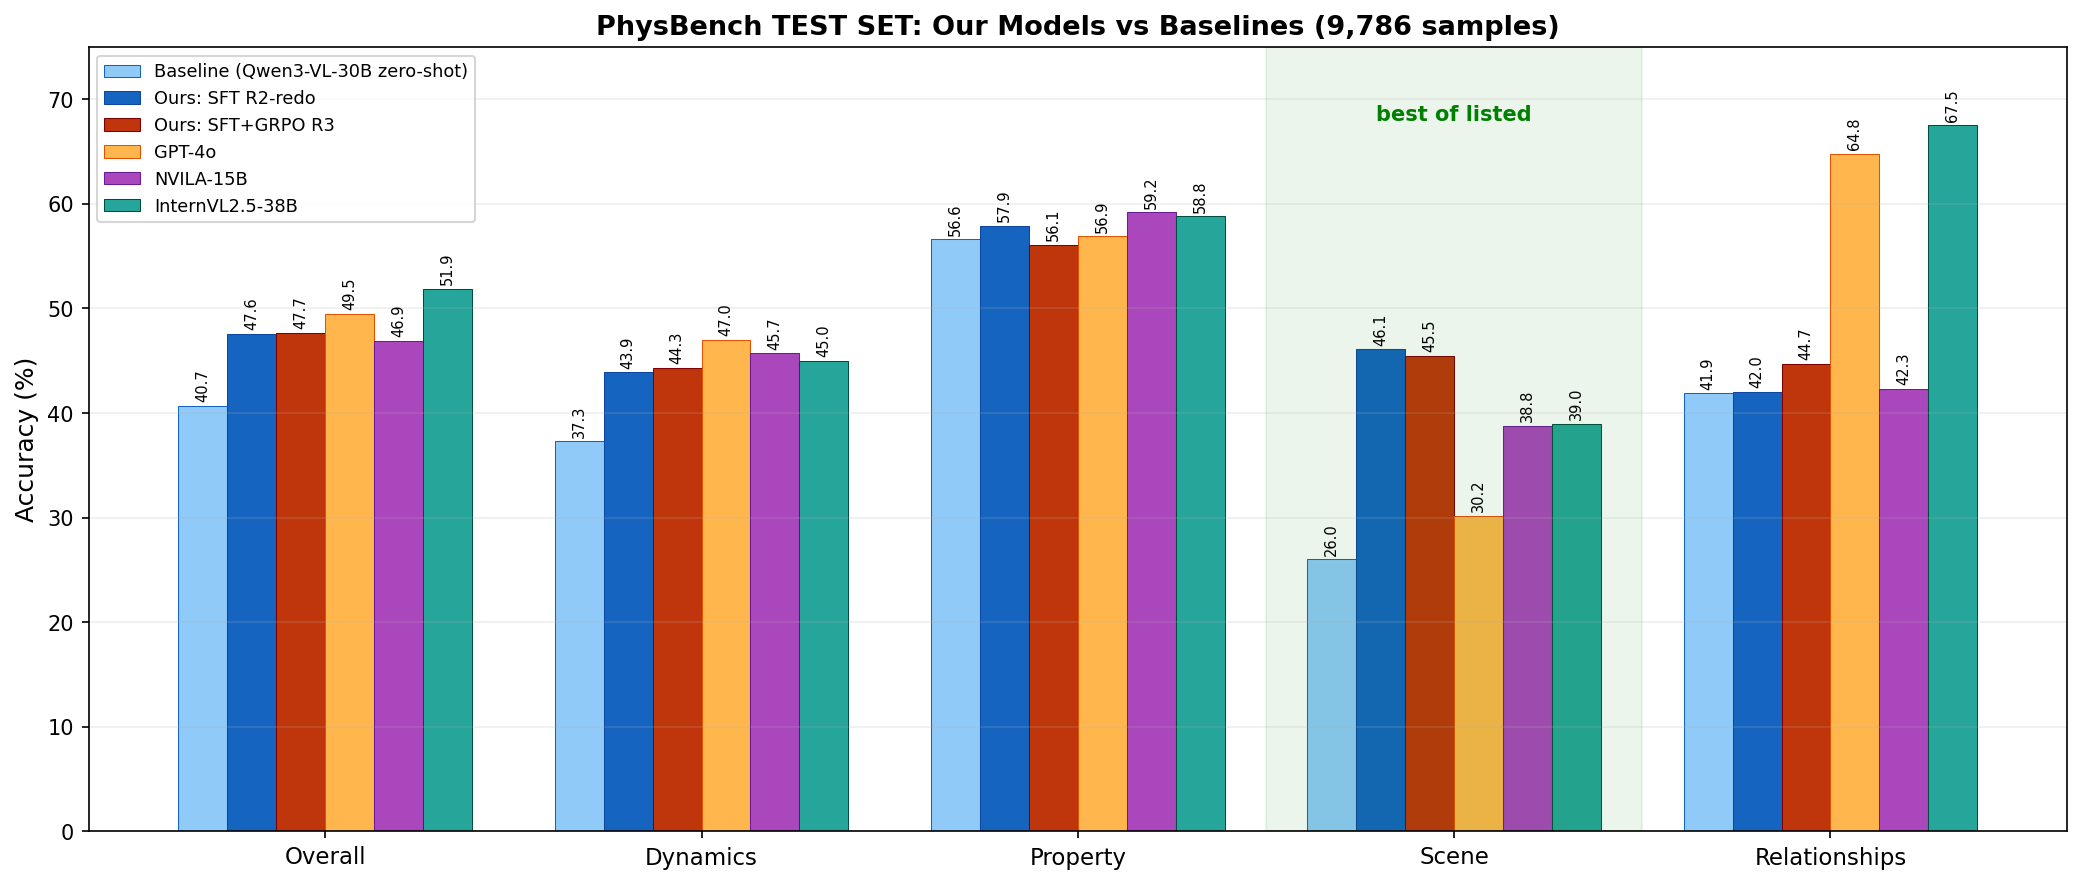
\includegraphics[width=0.92\linewidth]{figures/physbench_comparison.png}
\caption{PhysBench Test accuracy
($n{=}9{,}786$) for the un-tuned Qwen3-VL-30B baseline, our
PhysSim-VLM checkpoints (SFT R1, SFT R2-redo, GRPO R3), and three
public reference VLMs from the PhysBench leaderboard
(GPT-4o~\cite{gpt4o2024}, NVILA-15B~\cite{nvila2024},
InternVL2.5-38B~\cite{internvl2_5}). Our synthetic-only training
recipe lifts overall accuracy by ${+}6.9$pp at SFT R2-redo
(${+}7.0$pp at GRPO R3) and Scene by ${+}20.0$pp. Reference rows
are reproduced from the public PhysBench leaderboard and the
``best of listed'' annotation in the Scene column refers to the
four reference rows shown; for transparency we note that each
contributor's prompting and extraction conventions can affect
cross-row comparability.}
\label{fig:pbcompare}
\end{figure*}

Modern vision-language models (VLMs) achieve strong results on
broad multimodal benchmarks but remain unreliable on
\emph{physics-grounded} visual reasoning: predicting whether a stack
will topple, which of two fluids is more viscous, or where a rolling
ball will end up. Closing this gap with human-labelled physics data
is expensive: physics annotation requires domain expertise, scales
poorly, and the few existing physics-VLM benchmarks (PhysBench~\cite{physbench2024},
SeePhys~\cite{seephys2025}, PhysReason~\cite{physreason2025})
report a long tail of subtasks where even frontier models leave
substantial headroom. This bottleneck
motivates a methodological question: can a VLM learn physics from
a sandbox? We fine-tune on synthetic scenes
of coloured boxes, spheres, and cylinders interacting in a
simulator, then test on PhysBench real-world photos and videos.
The source data is deliberately stripped down (geometric objects,
minimal visual detail, no people, no clutter), while the target
data is naturalistic and visually complex. If PhysBench accuracy
improves, that suggests the model learned transferable physical
regularities instead of matching synthetic appearance.

Training uses minimalist MuJoCo rigid-body and PhiFlow
fluid scenes with 2--5 primitive shapes under basic mechanics. Outputs
are \textbf{free-text} answers (for example
\texttt{<answer>left</answer>} and \texttt{<answer>2</answer>}), not
A/B/C/D labels. We fine-tune Qwen3-VL-30B~\cite{qwen3vl2025} with a
three-stage LoRA~\cite{lora2022} recipe on the public Tinker
service~\cite{tinker2025}: SFT~R1 on $12{,}023$ MuJoCo scenes, SFT
R2-redo on $2{,}574$ corrected PhiFlow and categorical scenes, then
GRPO~R3 on $1{,}200$ scenes with simulator-verifiable
rewards~\cite{deepseekmath2024}. Evaluation uses
PhysBench~\cite{physbench2024} ($n{=}9{,}786$, disjoint
scene/style/format) and ScienceQA-Physics ($n{=}425$) for
off-distribution transfer.

PhysBench accuracy improves by $+6.9$pp after synthetic-only SFT,
with broad gains across subtasks; the detailed domain, mode, and
stage-wise analysis is presented in
Sections~\ref{sec:exp}--\ref{sec:analysis}.

\paragraph{Contributions.}
\begin{itemize}\itemsep0.05em
  \item A reproducible, fully synthetic training pipeline
        ($15{,}797$ scenes used in training: $14{,}597$ for SFT and
        $1{,}200$ for GRPO, drawn from a $16{,}617$-scene candidate
        pool after quality filtering; $8$ task families;
        MuJoCo~+~PhiFlow) that uses no human annotation, no
        local GPU, and under $\$30$ of hosted-API credits for all
        training stages combined ($\$4$ to $\$5$ per single SFT
        epoch).
  \item Cross-distribution and cross-format evidence: free-text
        training on synthetic MuJoCo and PhiFlow scenes improves
        PhysBench by $+6.9$pp, and the gain pattern follows the task
        families seen during training. The generated dataset targets a
        selected subset of physics properties with direct and indirect
        links to PhysBench, not all PhysBench classes.
  \item A detailed analysis that separates three effects in the lift:
        format commitment, latent-skill recovery, and physics
        capability gains, showing that most of the net improvement is
        explained by commitment/recovery, with smaller but measurable
        new-capability gains,
        and checking (\S\ref{sec:rescue}) whether the observed gain
        primarily reflects physics competence, not answer-format
        effects.
  \item An item-level comparison of the verifiable-reward (GRPO~R3)
        stage against the preceding SFT stage, showing that GRPO does
        not significantly improve overall accuracy ($+0.08$pp,
        within Wilson CI) but redistributes errors across mode and
        domain, with concentrated gains in
        \texttt{general:relationships} and losses in
        \texttt{image\&video:property}; we include the full shift
        pattern in the paper.
  \item A data-fidelity probe at both the SFT and RL stages showing
        that physically accurate fluid supervision improves PhysBench
        while a deliberately low-fidelity variant of the same corpus
        does not, providing evidence that transfer is driven by the
        physical quality of the synthetic training signal rather than
        by surface artefacts of the data.
\end{itemize}

\section{Related Work}
\label{sec:related}

\paragraph{Physics benchmarks for VLMs.}
We evaluate on two complementary benchmarks. \textbf{PhysBench}
\cite{physbench2024} provides $9{,}786$ test items across four physics
domains (Property, Relationships, Scene, Dynamics) and three modes
(image-only, image\&video, text-only ``general'') and is in-domain to
our evaluation target while remaining visually out-of-domain from
our synthetic training distribution. \textbf{ScienceQA-Physics}
\cite{scienceqa2022} provides K-12 textbook-style physics QA and is
used here as a strict off-distribution transfer probe.

\paragraph{Synthetic data, intuitive physics, and simulator-derived supervision.}
Synthetic, simulator-rendered scenes have a long history as probes for
visual physics reasoning: IntPhys~\cite{intphys2018} and
Physion~\cite{physion2021} measure intuitive-physics judgements (object
permanence, support, dynamics prediction) on controlled rigid-body
clips. CLEVRER~\cite{clevrer} introduces collision-event reasoning
from physics-engine rollouts; ContPhy~\cite{contphy2024} extends this
to continuum bodies (cloth, fluid) for video QA; PhysGen~\cite{physgen2024}
uses rigid-body physics to ground image-to-video generation. A
parallel line evaluates whether generated video itself respects
physical laws (VideoPhy~\cite{videophy2024}, PhyWorld~\cite{phyworld2024}).
Closest to our setting, Synthetic Vision~\cite{syntheticvision2024}
fine-tunes a VLM on simulator-generated QA pairs and measures a
stability-prediction probe; we differ in using free-text
\texttt{<answer>} labels read directly from simulator state, in
covering both rigid-body and continuum-fluid scenes, and in measuring
transfer on the broader PhysBench benchmark. The broader idea of
using physical laws and constraints as a label-free training
signal~\cite{labelfreephysics2017} extends here to instruction-tuned
VLMs, where both rendered frames and the numeric simulator state
are consumed as ground truth, removing caption- or QA-pair labelling.

\paragraph{Reinforcement learning with verifiable rewards.}
Recent work on reasoning-LLMs replaces preference-labelled rewards
with programmatically checkable ones (e.g.\ unit tests, exact-match
math answers)~\cite{deepseekr12025,deepseekmath2024}, removing the
dependence on human raters. We adopt
GRPO~\cite{deepseekmath2024}, a critic-free PPO~\cite{ppo2017}
variant that estimates per-token advantages from a group of
on-policy rollouts, because it is sample-efficient and removes
the value-network cost. Concurrent work on REINFORCE-style RL for
RLHF~\cite{rloo2024} reaches similar conclusions about the cost
asymmetry of value-network methods. Our reward is the simulator
state itself, so the verifiable-reward criterion is satisfied
without human preference labels or learned reward models.

\paragraph{Parameter efficient fine-tuning of large VLMs.}
End-to-end fine-tuning of large multimodal models is typically
expensive in GPU-hours and memory; we instead use LoRA~\cite{lora2022}
on
Qwen3-VL-30B with rank-16 adapters for SFT and rank-64 adapters
for GRPO ($\sim 0.4$--$1.7\%$ of backbone parameters), trained on
the public Tinker LoRA service in under $12$ wall-clock hours
total across both SFT rounds and the GRPO run.

\section{Method}
\label{sec:method}

\subsection{Synthetic Data Generation: Toy Primitives Only}
\label{sec:data}

The training distribution is deliberately minimalist: every
training scene contains 2--5 geometric primitives (boxes,
spheres, cylinders, capsules) on a uniform background, with random
masses, sizes, colours, initial velocities and lighting. There are no
real-world textures, no humans, no animals, no household objects, and
no scene clutter. The test distribution (PhysBench) is the
opposite: in-the-wild photos and videos of real-world physical
events, people, fluids in containers, mechanical apparatus,
laboratory setups. The cross-distribution gap is large by
construction; whether the model still transfers is what we test.

We generate a candidate pool of $16{,}617$ scenes using two
simulators: $12{,}023$ rigid-body scenes from
MuJoCo~\cite{mujoco2012} (time-to-collision, projectile trajectory,
pile stability, manipulation, throwing, collision) and $4{,}594$
continuum scenes from PhiFlow~\cite{phiflow2020} (with corrections
to viscosity, direction, and fluid-level estimators). After quality
filtering and deduplication, $14{,}597$ scenes are used in
training: all $12{,}023$ MuJoCo scenes (SFT R1) plus a
$2{,}574$-scene PhiFlow + categorical-comparison subset (SFT
R2-redo). The remaining PhiFlow scenes were excluded because they did
not pass the Gaussian-density quality check or duplicated existing
direction or viscosity prompts. PhiFlow simulates fluid as discrete particles;
we render each scene by depositing particle mass onto a
$256{\times}256$ density grid and applying a SciPy Gaussian filter
(\texttt{scipy.ndimage.gaussian\_filter}, $\sigma=7$ pixels) so the
result reads as a smooth, connected fluid body rather than a
particle cloud. Each scene yields (i) a $1$ to $3$s RGB rollout
sampled at $8$ frames, (ii) a single ``cover'' image, and (iii) all
simulator state variables that constitute the physical ground
truth. From the same simulator state we automatically construct
five categorical comparison families (mass/size, viscosity, level,
direction, count/viewpoint), which together with the three
continuous MuJoCo families (TTC, trajectory) and one stability family
yield \emph{eight} training-task families overall.

For each scene we emit a teacher-forced answer in
\textbf{free-text} form, wrapped in
\texttt{<answer>...</answer>} tags. Discrete tasks use a short
free-text categorical token (e.g.\ \texttt{<answer>left</answer>},
\texttt{<answer>fluid b</answer>}, \texttt{<answer>stable</answer>});
continuous tasks use a numeric scalar (e.g.\ time-to-collision in
seconds, viscosity rank on $[0,1]$). No training answer is in
A/B/C/D format; the model is never shown the MCQ letter convention
used by PhysBench evaluation. The supervision is read
directly from simulator state, with no human in the loop.
Table~\ref{tab:trainsamples} shows representative (prompt,
ground-truth) pairs from each of the eight training-task families.

\paragraph{No data leakage.} The training distribution is disjoint
from any PhysBench, ScienceQA, or other public physics-benchmark
item: scenes are sampled de-novo from MuJoCo and PhiFlow with
randomised geometry, masses, viscosities, lighting, and camera
poses. No PhysBench image, video, or question text appears in our
training corpus, and the rendering style (single-camera MuJoCo
renderer at $640{\times}480$; SciPy-smoothed PhiFlow density at
$256{\times}256$) is visually distinct from the heterogeneous
in-the-wild PhysBench imagery (Fig.~\ref{fig:physbench_grid}).
Additional training scenes covering the categorical-comparison
families used in SFT R2-redo are shown in Fig.~\ref{fig:compare_grid}.
Generalisation across this train-test domain gap is therefore part
of what we measure.

\begin{table}[t]
\caption{Representative (prompt, ground-truth) pairs from selected
training-task families (we use eight families overall: three
continuous MuJoCo plus five categorical). Prompts are emitted with
the \texttt{<reasoning>...</reasoning><answer>...</answer>} schema
shown; ground-truth answers and rationales are derived directly
from simulator state.}
\label{tab:trainsamples}
\centering
\footnotesize
\begin{tabular}{p{0.95\linewidth}}
\toprule
\textbf{TTC (MuJoCo, continuous):}\\
\textit{Prompt}: ``Two objects are moving in this 0.6-second video.
Object A: purple sphere. Object B: white sphere. When will they
collide? Give seconds from the start of the video.''\\
\textit{GT}: \texttt{<answer>0.78</answer>} (closing speed gives
$0.22$s remaining after clip ends).\\
\midrule
\textbf{Trajectory (MuJoCo, continuous):}\\
\textit{Prompt}: ``Watch this projectile's initial flight (0.3s
shown). Predict the final resting position.''\\
\textit{GT}: \texttt{<answer>x=1.61, y=0.02</answer>} (parabolic
extrapolation from 4-frame clip).\\
\midrule
\textbf{Stability (MuJoCo, categorical):}\\
\textit{Prompt}: ``Analyze this stack: base orange box (0.26\,m),
layer 2 blue sphere (0.18\,m). Will it remain stable or topple?''\\
\textit{GT}: \texttt{<answer>stable</answer>} (max observed
displacement 0.0017\,m).\\
\midrule
\textbf{Fluid direction (PhiFlow, categorical):}\\
\textit{Prompt}: ``A body of fluid (blue) is released. In which
primary direction does the fluid move? Options: left, right, down.''\\
\textit{GT}: \texttt{<answer>left</answer>} (centre-of-mass
displacement $\Delta x{=}{-0.54}$, $\Delta y{=}{-0.34}$\,m).\\
\midrule
\textbf{Fluid viscosity (PhiFlow, categorical):}\\
\textit{Prompt}: ``Fluid A (blue, left) and Fluid B (orange, right)
in the same container. Which is more viscous?''\\
\textit{GT}: \texttt{<answer>fluid b</answer>} (B remains compact
across the sequence; A spreads into curved streams).\\
\bottomrule
\end{tabular}
\end{table}

\begin{figure}[t]
\centering
\setlength{\tabcolsep}{1pt}
\renewcommand{\arraystretch}{0.6}
\begin{tabular}{ccc}
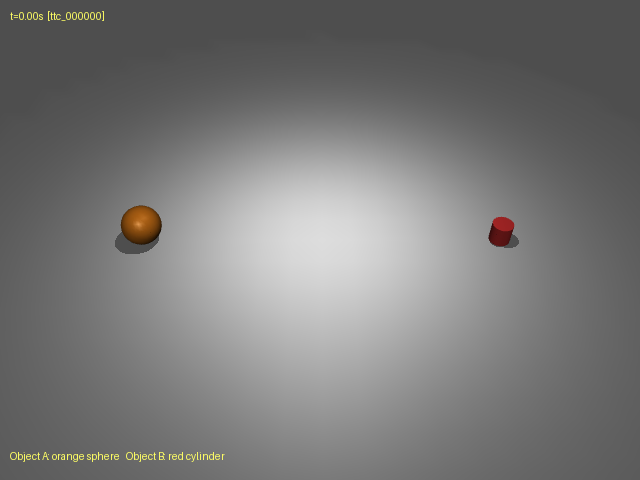
\includegraphics[width=0.30\linewidth,height=1.6cm,keepaspectratio]{samples/mujoco_ttc_frame0.png} &
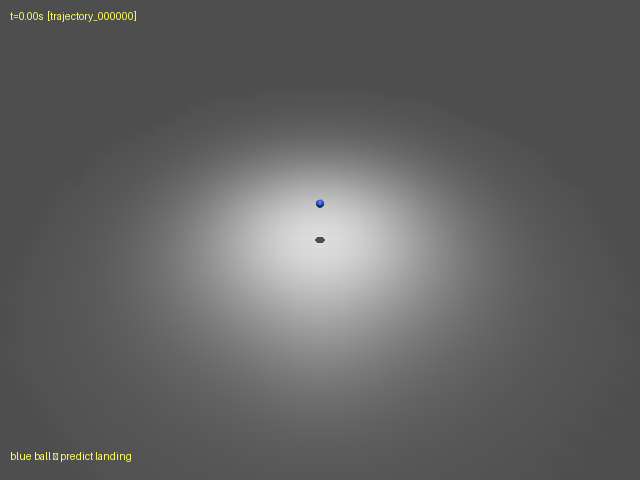
\includegraphics[width=0.30\linewidth,height=1.6cm,keepaspectratio]{samples/mujoco_trajectory_frame0.png} &
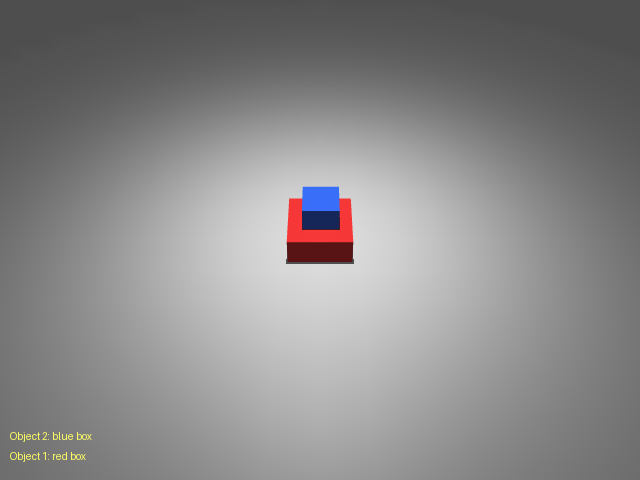
\includegraphics[width=0.30\linewidth,height=1.6cm,keepaspectratio]{samples/mujoco_stability.png} \\
\multicolumn{3}{c}{\footnotesize MuJoCo: TTC / trajectory / stability}\\[3pt]
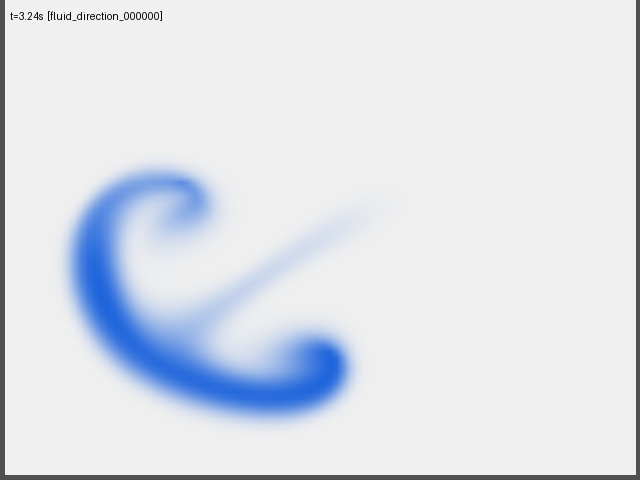
\includegraphics[width=0.30\linewidth,height=1.6cm,keepaspectratio]{samples/phiflow_corrected/dir_left.png} &
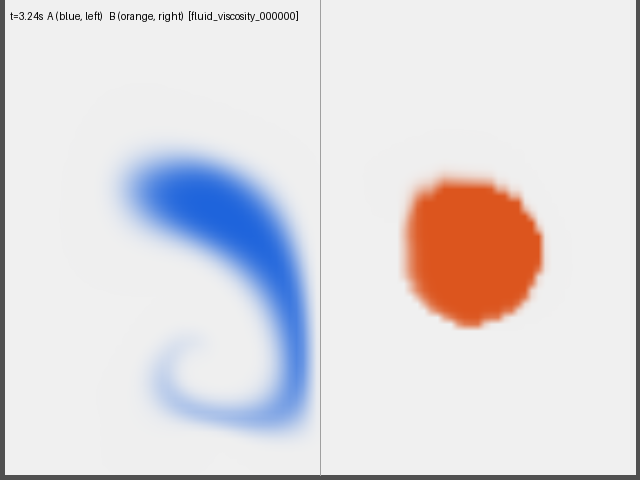
\includegraphics[width=0.30\linewidth,height=1.6cm,keepaspectratio]{samples/phiflow_corrected/visc_high.png} &
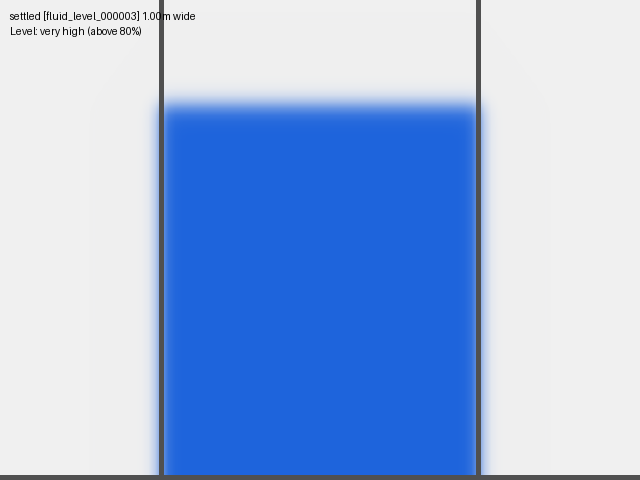
\includegraphics[width=0.30\linewidth,height=1.6cm,keepaspectratio]{samples/phiflow_corrected/level_high.png} \\
\multicolumn{3}{c}{\footnotesize PhiFlow: direction / viscosity / level}\\
\end{tabular}
\caption{Sample training scenes (one per family). MuJoCo rigid-body
scenes (top) and PhiFlow continuum-fluid scenes (bottom). Full
per-task grids in App.~\ref{sec:appendix-samples}; PhysBench test
scenes in App.~\ref{sec:appendix-samples}, Fig.~\ref{fig:physbench_grid}.}
\label{fig:dataset_overview}
\end{figure}


Figure~\ref{fig:dataset_overview} previews one scene per family;
full per-task grids and PhysBench test scenes are in
Appendix~\ref{sec:appendix-samples}
(Figs.~\ref{fig:mujoco_grid}--\ref{fig:physbench_grid}).

\subsection{Supervised Fine-Tuning}
\label{sec:sft}

We fine-tune Qwen3-VL-30B-A3B-Instruct with LoRA (rank 16, all linear
projections) using teacher-forced answers. All training is performed
on the public Tinker LoRA service~\cite{tinker2025}, which exposes
a managed sampling and gradient endpoint and removes the need for
local GPU infrastructure. We run two SFT rounds in a sequential
curriculum (the second resumes from the first):

\begin{itemize}\itemsep0.05em
  \item \textbf{SFT R1}: 12{,}023 MuJoCo scenes, 1 full epoch
        (751 steps, $\sim 3.7$ wall hours). Covers TTC,
        trajectory, and stability tasks.
  \item \textbf{SFT R2 (low-fidelity fluid, data-fidelity probe)}:
        resumed from R1 on a low-fidelity PhiFlow corpus in which
        $\sim$29\% of fluid scenes lacked the Gaussian density
        smoothing described in \S\ref{sec:data} and carried noisy
        viscosity/direction/level targets. We use this run as an
        intentional data-fidelity probe: if the model is genuinely
        learning physics, training on physically less accurate
        supervision should not improve PhysBench, whereas training on
        physically accurate supervision should. SFT R2 indeed shows
        no improvement on the Dynamics domain on a partial test eval,
        motivating a regeneration of the fluid corpus with corrected
        physics.
  \item \textbf{SFT R2-redo (corrected physics)}: same recipe as SFT
        R2 but on the corrected, Gaussian-smoothed fluid data,
        comprising $2{,}574$ scenes, 644 steps, $\sim 3.9$ wall
        hours, again resuming from R1 weights. With physically
        accurate supervision the model improves on the targeted
        domains (Tables~\ref{tab:ablation}--\ref{tab:leaderboard}),
        completing the data-fidelity contrast and providing evidence
        that the gain tracks the physical quality of the training
        signal.
\end{itemize}

The two-stage curriculum lets us isolate the contribution of the rigid-body
and continuum-body data sources in our ablation
(Table~\ref{tab:ablation}).

\paragraph{Why a single epoch per round.} Each round uses exactly
one pass. The SFT R1 mean training loss bottoms at $0.076$ around
step $400$ of $751$ and then drifts up to $0.136$ by end-of-epoch
(Fig.~\ref{fig:trainloss}), which already looks like mild
overfitting on the \texttt{<answer>...</answer>} schema. Smoke
runs of a second SFT epoch confirmed this: rank-16 adapters began
memorising exact numeric answers on the continuous tasks (TTC,
trajectory) instead of the input-to-answer mapping. The same
behaviour reappears at the RL stage: an exploratory GRPO~Run~2
epoch~2 ($475$ additional steps from the Ep1 checkpoint) regressed
val accuracy from $65.8\%$ to $64.3\%$ despite a final training
reward of $0.84$, a clear reward-hacking signature on the small
($n{=}951$) GRPO scene pool. The SFT~R2 data-fidelity probe above
further shows that a second pass on low-fidelity supervision does
not transfer to PhysBench, so we keep one epoch per stage to stay
auditable.

\subsection{Reinforcement Learning with Verifiable Rewards (GRPO)}
\label{sec:grpo}

SFT pushes the model toward the right answer string. It does not push
it toward better physical reasoning along the way, since cross-entropy
only sees the final answer tokens. We add a third stage that uses
GRPO~\cite{deepseekmath2024} with simulator-verifiable rewards to see
whether RL can close that gap.
We adopt this method because it forgoes a learned value network, which
is relevant for our small-budget setting, and replaces it with a
within-prompt baseline. Concretely, for each prompt we draw $G$
on-policy completions, score each with a scalar reward $r_i$, and
assign every token of completion $i$ the group-normalised advantage
\[
\hat{A}_{i,t} = \frac{r_i - \mathrm{mean}(\{r_j\}_{j=1}^{G})}
                     {\mathrm{std}(\{r_j\}_{j=1}^{G})}
\]
which is then plugged into the PPO~\cite{ppo2017} clipped surrogate
objective with a KL penalty to the SFT R2-redo reference policy.

\paragraph{Reward design.} The reward is a weighted sum of two
simulator-verifiable terms: a \emph{physics correctness} reward
($w_{\text{phys}}{=}0.95$) that scores the parsed answer against
simulator state (exact-match for MCQ, exponential-decay for
continuous targets such as TTC and trajectory), and a small
\emph{format} reward ($w_{\text{fmt}}{=}0.05$) that requires the
\texttt{<reasoning>...</reasoning><answer>...</answer>} schema. No
human preference labels are used.

\paragraph{Run~2 (low-fidelity fluid, RL data-fidelity probe).} An
initial GRPO run resumed from R2-redo on the same low-fidelity PhiFlow
corpus used in the SFT~R2 probe, providing a parallel data-fidelity
contrast at the RL stage. Consistent with the SFT~R2 observation,
training with physically less accurate supervision yields a $-1.2$pp
movement relative to R1 ($46.3\%$ vs.\ $47.5\%$) and $-1.4$pp relative
to R2-redo ($47.6\%$), with $481$ ($4.9\%$) of completions emitting
non-letter free text that the official extractor scored as empty.
Recovering these via a free-text-to-option matcher (\S\ref{sec:rescue})
restores most of the gap, indicating the change was largely a
format-collapse artefact, separable from physics capability. We
report this RL-stage data-fidelity probe as additional evidence that
training-signal quality matters for the RL stage as well, and as a
cautionary observation about reward shaping under formatting pressure.

\paragraph{Run~3 (corrected, GRPO R3).} The reported GRPO model
resumes from R2-redo on a corrected curriculum of $1{,}200$ scenes
that re-balances the corpus: $300$ static-image scenes (preventing
image-only regression) plus $900$ video scenes covering all
five direct-target families (TTC, trajectory, stability, fluid,
manipulation). Categorical prompts retain the same free-text
\texttt{<answer>...</answer>} schema used in SFT (no MCQ
re-wrapping), so the model's MCQ behaviour at evaluation time comes
entirely from the inline option list in each PhysBench question.
We use group size $G{=}4$, two groups per batch, temperature $0.7$,
max tokens $768$, KL penalty $0.04$, $300$ optimisation steps, and
rank-64 LoRA adapters
(\S\ref{sec:appendix-grpo} lists the full schedule;
Figs.~\ref{fig:grpo_reward} and~\ref{fig:grpo_coverage} show the
training-reward trajectory and the per-task data coverage).

\paragraph{What changes after GRPO?} GRPO~R3 does not significantly
improve overall accuracy over SFT~R2-redo ($47.7\%$ vs.\ $47.6\%$,
a delta of $+0.08$pp that sits well within Wilson 95\% CI overlap).
At the per-item level, GRPO~R3 newly rescues $761$ R2-wrong items and
newly loses $753$ R2-correct items: a near-even swap (net $+8$ items
out of $9{,}786$, $+0.08\%$). The swap is \emph{not} uniformly
distributed (Table~\ref{tab:r2_grpo_swap}); it concentrates in a few
mode--domain cells.

\begin{table}[t]
\caption{Item-level swap from SFT R2-redo to GRPO R3 ($n{=}9{,}786$
PhysBench Test). ``Gained'' = R2-redo wrong, GRPO R3 correct; ``Lost''
= R2-redo correct, GRPO R3 wrong. Rows ordered by $|$net$|$.}
\label{tab:r2_grpo_swap}
\centering
\footnotesize
\setlength{\tabcolsep}{4pt}
\begin{tabular}{llrrr}
\toprule
Mode & Domain & Gained & Lost & Net \\
\midrule
general      & relationships  & 276 & 213 & $+63$ \\
image\&video & property       & 60  & 129 & $-69$ \\
image\&video & dynamics       & 150 & 150 & $0$ \\
image\&video & scene          & 90  & 104 & $-14$ \\
image-only   & property       & 90  & 65  & $+25$ \\
image-only   & dynamics       & 42  & 42  & $0$ \\
\textit{other (4 cells)} &    & 53  & 50  & $+3$ \\
\midrule
\textbf{Total} &              & \textbf{761} & \textbf{753} & $\mathbf{+8}$ \\
\bottomrule
\end{tabular}
\end{table}

The pattern: GRPO rescues many \texttt{general:relationships} items
(text-heavy multi-image-option spatial-motion questions R2-redo
confuses), at the price of regressing on \texttt{image\&video:property}
(real-world object-attribute/count questions). For example, GRPO
\emph{rescues} idx~5099 (``If we want the brown pulley to rotate
clockwise, what can we do?''), R2-redo answers ``Increase the
mass of the brown cube'' (\xmark), GRPO produces an explicit
force/torque analysis and answers \textbf{D} (\cmark). It \emph{loses}
idx~4883 (fluid pass-through), R2-redo correct, GRPO becomes more
verbose but commits to a worse spatial inference. Net: GRPO on
$1{,}200$ scenes redistributes where the model commits without
consistently sharpening physics, so we report the per-domain swap in
Table~\ref{tab:r2_grpo_swap} as the main GRPO finding rather than an
accuracy lift.

\paragraph{Why GRPO did not significantly improve over SFT~R2-redo.}
Three issues explain the small overall delta. Coverage was thin:
Run~1's variance-conditioned sampling concentrated rollouts on
$\sim 195/15{,}714$ scenes ($1.2\%$); Run~2 fixed the concentration
(Fig.~\ref{fig:grpo_coverage}) but only on $951$ balanced scenes,
and Run~3 trains on $1{,}200$ ($\leq 30$ rollouts per (mode, task)
cell). On top of that, an exploratory Run~2 Epoch~2 ($475$ extra
steps) reached training reward $0.84$ while \emph{regressing} val
from $65.8$ to $64.3\%$, a clear case of overfitting scene-specific
shortcuts on the small fixed pool. And SFT had already absorbed the
bulk of the transferable signal, so GRPO can only sharpen items
where the SFT policy was already indecisive. Practitioners with
fixed compute should likely stop at SFT~R2-redo unless the GRPO
scene pool can be expanded substantially.

\section{Experiments}
\label{sec:exp}

\subsection{Targeted Categories and Mechanism of Impact}
\label{sec:targets}

Our eight training-task families were designed to load on three of
PhysBench's four physics domains. \emph{Direct} targets (training
labels mirror the test subtask) are: TTC, trajectory, fluid
direction/viscosity/level map to \textbf{Dynamics}; stability, mass/size
compare, fluid viscosity/level, counting (cardinality of objects)
map to \textbf{Property} (PhysBench groups counting under
\texttt{property:number}); viewpoint maps to \textbf{Scene}.
\emph{Indirect} targets (shared visual primitives or reasoning style,
no label-level overlap) include stability mapping to Property:attribute
and fluid direction mapping to Relations:motion. The text-only general
mode and the Relationships domain were not directly targeted by
label-level supervision in any family.

The largest test-set lifts in Table~\ref{tab:perdomain} fall on the
domains this mapping predicts: \textbf{Scene} $+20.0$pp (from $26.0$
to $46.1\%$ at SFT R2-redo, driven by viewpoint and format alignment),
\textbf{Dynamics} $+6.6$pp ($37.3$ to $43.9\%$ at R2-redo;
SFT~R1 alone reaches $44.4\%$/${+}7.1$pp, and the small
R1-to-R2-redo regression on Dynamics is itself within Wilson CI noise), driven by
TTC, trajectory, fluid tasks), and \textbf{Property} $+1.3$pp
(stability, mass/size). At the mode level: image\&video gains
$+12.7$pp at R2-redo (the modality our video rollouts match),
image-only is flat ($+0.3$pp at R2-redo, no static-image training),
and the un-targeted general mode regresses $-3.8$pp under SFT.
Indirectly, fluid-direction training lifts the Relations:motion
subtask even though our fluid labels never use relational language;
the shared cue is a moving body in a frame. ScienceQA-Physics
(\S\ref{sec:transfer}) was not targeted by any family and shows no
significant change: we did not train on textbook physics, and that
physics did not show up in the test.

\subsection{In-Distribution: PhysBench Test ($n{=}9{,}786$)}

\begin{table}[t]
\caption{PhysBench Test accuracy across pipeline stages
($n{=}9{,}786$, $T{=}0$, max\_tokens 512). $\Delta$ is vs.\ Baseline.
Inter-trained-checkpoint gaps (R1 vs.\ R2-redo vs.\ GRPO R3) lie
within overlapping Wilson 95\% CIs and should not be read as
significant; only gaps to Baseline are. GRPO Run~2 is the
data-fidelity probe trained on the low-fidelity fluid corpus
(\S\ref{sec:grpo}).}
\label{tab:ablation}
\centering
\footnotesize
\setlength{\tabcolsep}{4pt}
\begin{tabular}{lccccc}
\toprule
Stage & Overall & img-only & img\&vid & general & $\Delta$ \\
\midrule
Baseline      & 40.7 & 58.4 & 38.8 & 27.5 & n/a \\
SFT R1        & 47.5 & 58.5 & 50.2 & 27.2 & $+6.8$ \\
SFT R2-redo   & 47.6 & 58.7 & 51.5 & 23.8 & $+6.9$ \\
GRPO Run~2    & 46.3 & 56.3 & 49.2 & 26.1 & $+5.6$ \\
GRPO R3       & 47.7 & 59.5 & 50.1 & 27.6 & $+7.0$ \\
\bottomrule
\end{tabular}
\end{table}

\begin{table}[t]
\caption{Per-task-type accuracy on PhysBench Test. \textbf{Bold}
marks the best entry per column.}
\label{tab:perdomain}
\centering
\small
\begin{tabular}{lcccc}
\toprule
Stage & Dynamics & Property & Relations & Scene \\
\midrule
Baseline       & 37.3 & 56.6 & 41.9 & 26.0 \\
SFT R1         & 44.4 & 56.9 & 43.2 & 44.8 \\
SFT R2-redo    & 43.9 & \textbf{57.9} & 42.0 & \textbf{46.1} \\
GRPO Run~2     & \textbf{45.3} & 55.6 & 41.3 & 41.6 \\
\textbf{GRPO R3 (ours)} & 44.3 & 56.1 & \textbf{44.7} & 45.5 \\
\bottomrule
\end{tabular}
\end{table}

Tables~\ref{tab:ablation} and~\ref{tab:perdomain} report the main
result. The bulk of the gain ($+6.8$pp overall at SFT~R1 and $+20.0$pp
on Scene at SFT~R2-redo) comes from synthetic SFT alone. The biggest
moves live in the image\&video mode ($+12.7$pp at R2-redo) where our training
distribution most directly applies. The text-only ``general''
mode initially regresses by $-3.8$pp under SFT R2-redo
($27.5$ to $23.8\%$) and is then recovered by GRPO R3
($+3.8$pp over R2-redo, restoring it to $27.6\%$). GRPO R3 also
adds $+2.7$pp on Relationships ($42.0$ to $44.7\%$), a domain our
SFT corpus does not directly target, at the cost of small movements on
Property and Scene; the per-stage swap is detailed in
Table~\ref{tab:r2_grpo_swap}.

\begin{figure}[t]
\centering
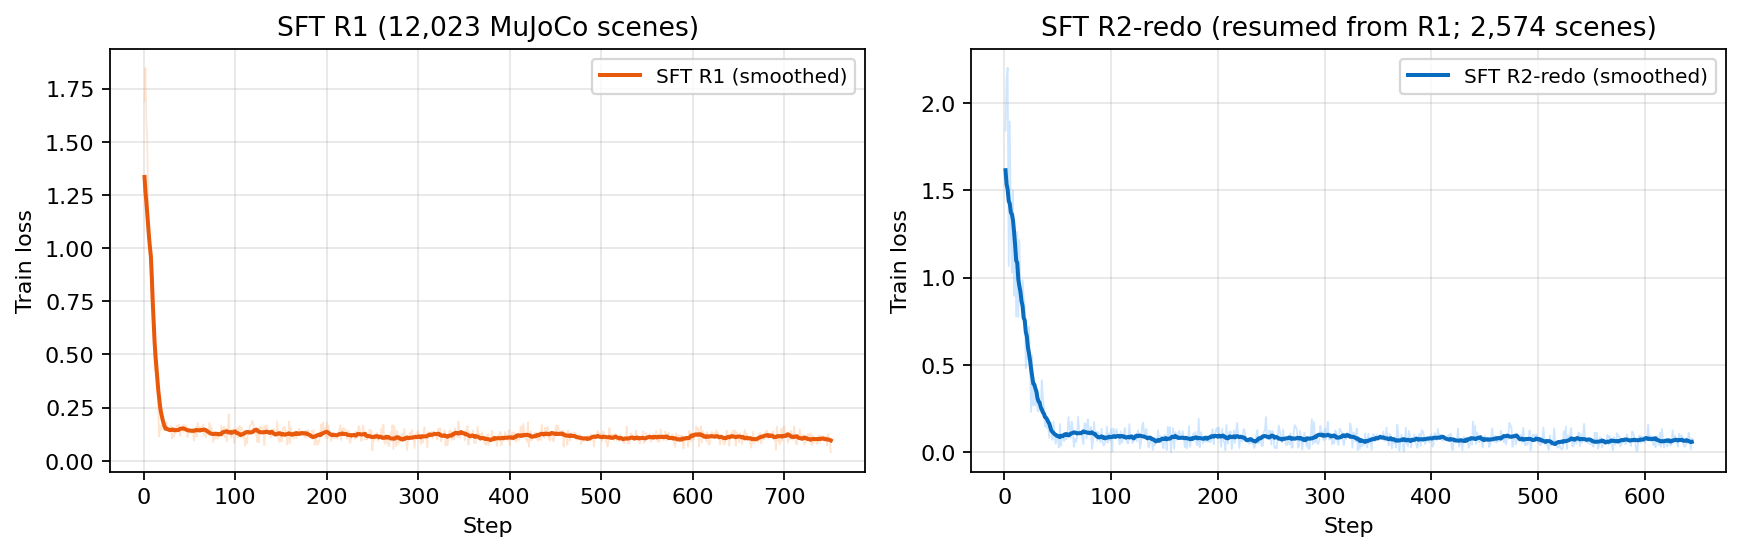
\includegraphics[width=\linewidth]{figures/training_loss_both.png}
\caption{SFT training loss for both rounds. \textbf{SFT R1} (orange,
$751$ steps over $12{,}023$ MuJoCo scenes) converges in one epoch.
\textbf{SFT R2-redo} (blue, $644$ steps over $2{,}574$ scenes)
resumes from the R1 weights and is trained on the corrected
PhiFlow continuum data plus the eight categorical comparison tasks.
Loss values are not directly comparable across rounds because the
two corpora differ in token length and label format.}
\label{fig:trainloss}
\end{figure}

\subsection{Per-Domain Specialisation}

\begin{table}[t]
\caption{Position on the public PhysBench leaderboard (29-model
snapshot, 2026-04-01)~\cite{physbench2024}, per physics domain.
Reference rows (GPT-4o~\cite{gpt4o2024}, InternVL2.5-78B/38B,
InternVL2-76B~\cite{internvl2_5}, NVILA-15B~\cite{nvila2024}) are
reproduced from the public PhysBench leaderboard under each
contributor's evaluation conventions; see Fig.~\ref{fig:pbcompare}
for the comparability note.}
\label{tab:leaderboard}
\centering
\footnotesize
\setlength{\tabcolsep}{4pt}
\begin{tabular}{lcccc}
\toprule
Model & Prop. & Rel. & Scene & Dyn. \\
\midrule
GPT-4o                  & 56.91 & 64.80 & 30.15 & \textbf{46.99} \\
InternVL2.5-78B         & \textbf{60.32} & 62.13 & 37.32 & 46.11 \\
InternVL2.5-38B         & 58.77 & \textbf{67.51} & 39.04 & 45.00 \\
NVILA-15B               & 59.16 & 42.34 & 38.78 & 45.72 \\
InternVL2-76B           & 57.65 & 52.43 & 38.07 & 40.12 \\
\midrule
Qwen3-VL-30B (base)     & 56.60 & 41.90 & 26.00 & 37.30 \\
\textbf{Ours (R1)}      & 56.90 & 43.20 & 44.80 & 44.40 \\
\textbf{Ours (R2-redo)} & 57.90 & 42.00 & 46.10 & 43.90 \\
\textbf{Ours (GRPO R3)} & 56.10 & 44.70 & 45.50 & 44.30 \\
\bottomrule
\end{tabular}
\end{table}

We report the leaderboard rows as evidence that our synthetic
pipeline transfers to a public physics benchmark. Reference rows are
reproduced from the public PhysBench leaderboard, so reviewers should
treat the listing as situating our results among published numbers
under each contributor's evaluation conventions. Two patterns are
consistent across the listing. On Scene, the dimension our MuJoCo
data targets most directly, our trained models score $44.8$--$46.1$,
in the same range as the listed reference rows. On Relationships,
where our training data does not contain relational annotation, gains
concentrate on the directly targeted Property/Dynamics/Scene domains.

\paragraph{Why the Scene domain moves so much.} The baseline scores
$26.03\%$ on Scene, near the $25\%$ random-guess floor, while the
extractor still finds a letter in $96.6\%$ of baseline responses
(\S\ref{sec:rescue}); the per-subtask shifts are visualised in
Fig.~\ref{fig:dynimp}. Two SFT effects drive the Scene jump. The
model stops hedging across options and commits to one, dropping
unparseable ``other-wrong'' responses from $23\%$ to $7\%$. On top
of that, multi-camera viewpoint training (camera pose as label)
directly lifts Scene\texttt{:viewpoint} by $+23.6$pp ($n{=}1008$).
Two large non-targeted subtask gains, Scene\texttt{:air}
($+33.3$pp, $n{=}42$) and Scene\texttt{:temperature} ($+41.4$pp,
$n{=}58$), look like the same decisiveness effect surfacing latent
baseline ability that the extractor previously did not surface; we
did not train on air or temperature. The Scene-domain lift is
therefore part true new skill (viewpoint), part recovery of latent
baseline knowledge.

\begin{figure}[t]
\centering
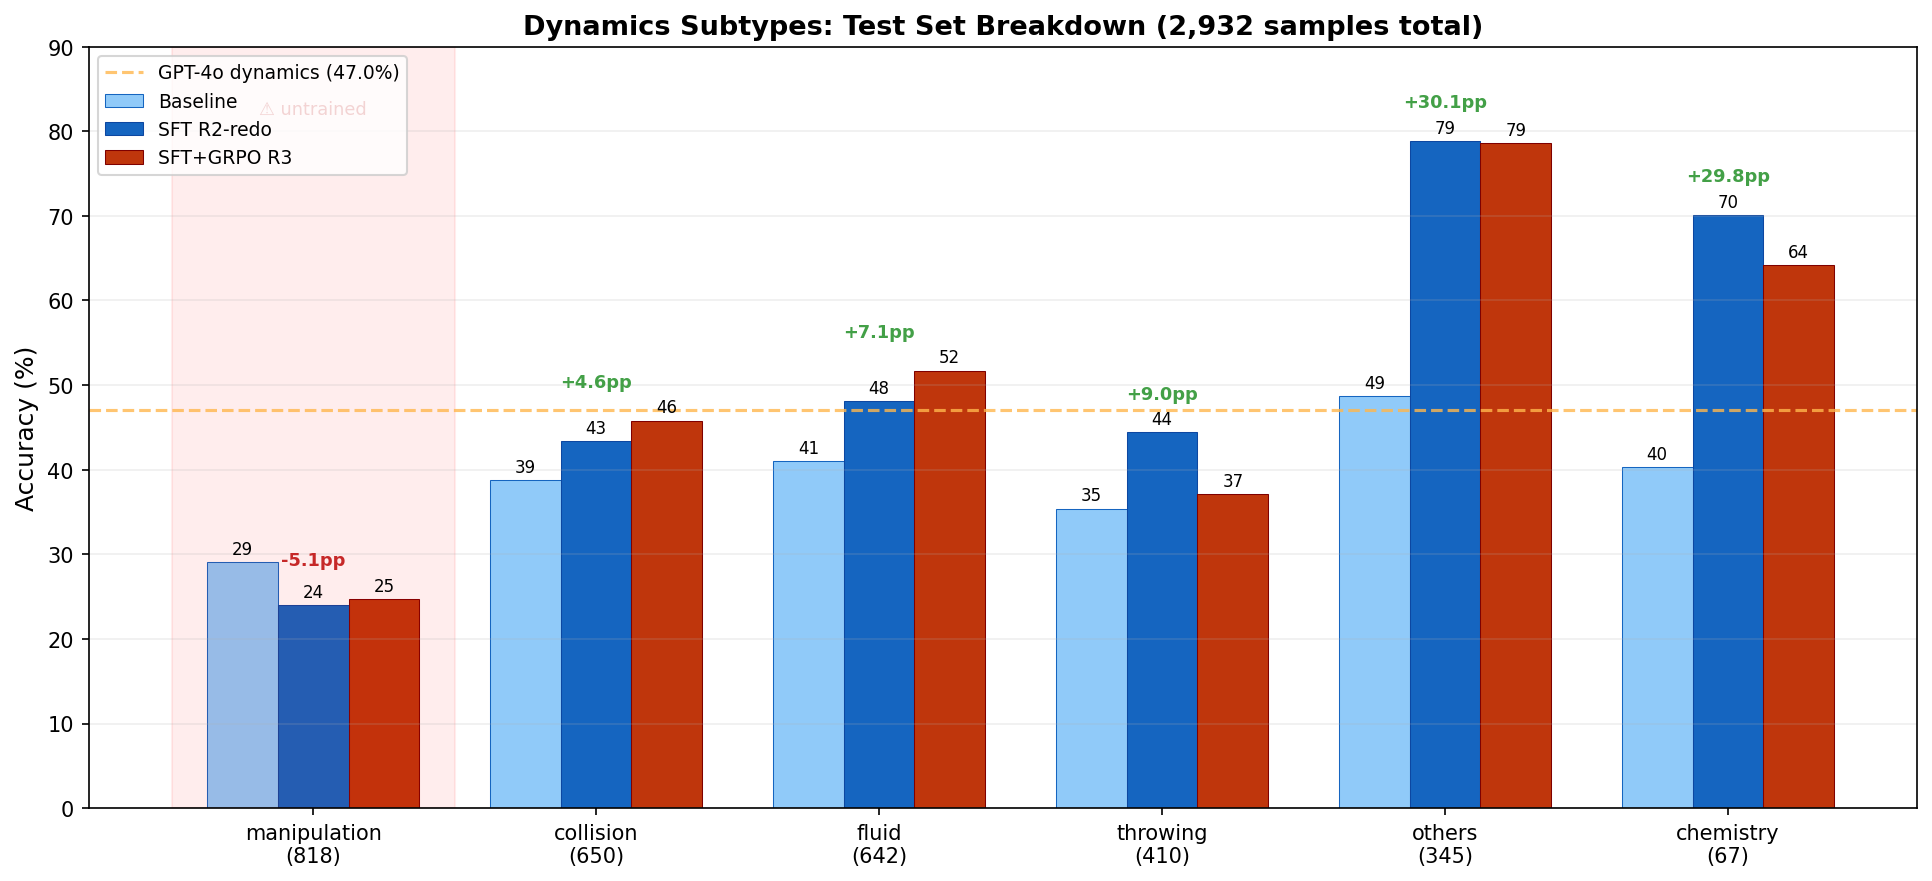
\includegraphics[width=\linewidth]{figures/dynamics_improvement.png}
\caption{Per-subtask improvement of SFT R2-redo over the baseline on
Dynamics and Scene subtasks. Largest jumps: Scene \texttt{air}
($+33.3$pp), \texttt{viewpoint} ($+23.6$pp), \texttt{temperature}
($+41.4$pp); Dynamics \texttt{chemistry} ($+29.9$pp),
\texttt{fluid} ($+7.2$pp), \texttt{collision} ($+4.4$pp).}
\label{fig:dynimp}
\end{figure}

\subsection{Off-Distribution Transfer: ScienceQA-Physics}
\label{sec:transfer}

To probe whether the gains are physics-general or PhysBench-specific,
we evaluate on the vision-essential subset of ScienceQA-Physics
($n{=}425$, $\geq 1$ image, K-12 textbook). SFT R2-redo scores
$79.53\%$ ($338/425$, Wilson 95\% CI~\cite{wilson1927}
$[75.44, 83.09]$) versus baseline $84.00\%$
($357/425$, $[80.21, 87.18]$). A two-proportion z-test gives
$z=-1.69$ ($p=0.09$). The test is \textbf{underpowered}: at
$n{=}425$ it detects a true $-4.5$pp effect with only $\sim 50\%$
power. The result is therefore consistent with both no transfer and
a small drop in K-12 textbook physics; a larger off-distribution
benchmark would be needed to tell the two apart. Either way, we have
no positive evidence that the recipe transfers beyond PhysBench.

\section{Analysis}
\label{sec:analysis}

\subsection{Failure-Mode Taxonomy}

We bucket every one of the $9{,}786$ predictions per checkpoint into
exactly one of nine response-shape categories
(Table~\ref{tab:failures}).

\begin{table}[t]
\caption{Failure-mode taxonomy on PhysBench Test ($n{=}9{,}786$ per
column). Numbers are absolute counts; percentages of the column total
in parentheses. Buckets are assigned in priority order
(off-by-1 MCQ first, then terse-wrong-letter on remaining items, then
verbose categories), so each item appears in exactly one row but the
\emph{shape categories} are not mutually exclusive in the underlying
behaviour (e.g.\ a terse single letter that is off-by-one is counted
as off-by-1 MCQ, not terse-wrong-letter).}
\label{tab:failures}
\centering
\scriptsize
\setlength{\tabcolsep}{3pt}
\begin{tabular}{lcccc}
\toprule
Mode & Base. & R1 & R2-redo & GRPO R3 \\
\midrule
correct              & 3984 (40.7) & 4649 (47.5) & 4662 (47.6) & \textbf{4670 (47.7)} \\
off-by-1 MCQ         & 2685 (27.4) & 2244 (22.9) & 2315 (23.7) & 2268 (23.2) \\
other wrong          & 2256 (23.1) & 891 (9.1)   & 725 (7.4)   & 924 (9.4)   \\
wrong w/ physics     & 611 (6.2)   & 101 (1.0)   & 57 (0.6)    & 183 (1.9)   \\
terse wrong letter   & 149 (1.5)   & 1014 (10.4) & 1048 (10.7) & 974 (10.0)  \\
terse wrong          & 1 (0.0)     & 873 (8.9)   & 979 (10.0)  & 766 (7.8)   \\
empty response       & 89 (0.9)    & 0 (0.0)     & 0 (0.0)     & 0 (0.0)     \\
unparseable          & 11 (0.1)    & 14 (0.1)    & 0 (0.0)     & 1 (0.0)     \\
refusal              & 0           & 0           & 0           & 0           \\
\bottomrule
\end{tabular}
\end{table}

The dominant failure mode at every stage is \emph{off-by-one MCQ},
a parseable single-letter response in $\{$A,B,C,D$\}$ that
disagrees with the gold letter by exactly one position in option
order ($23$ to $27\%$ of all responses, $43$ to $46\%$ of all
failures); the gap is one of discrimination between adjacent
options, not absent physics knowledge. SFT sharply collapses the
``verbose-but-wrong-with-physics'' mode ($6.2\%$ to $0.6\%$): the
model stops producing long, fluent, wrong explanations. It also
introduces a new failure mode, terse wrong answers ($1.5\%$ to
$10.7\%$), as the model adopts the short teacher-forced answer
style.

\subsection{Chain-of-Thought Length and Physics Vocabulary}
\label{sec:cot}

Chain-of-thought prompting~\cite{cot2022} is the standard lever for
eliciting step-by-step reasoning from instruction-tuned LLMs. We
analyse the post-SFT response length and lexical content as a proxy
for whether SFT changes the \emph{shape} of model reasoning, not just
the final letter.

\begin{table}[t]
\caption{Response-length and physics-vocabulary statistics on
PhysBench Test. Density = curated physics-vocabulary token fraction
$\times 100$.}
\label{tab:cot}
\centering
\small
\begin{tabular}{lccc}
\toprule
Checkpoint & Mean len. & Physics dens. & $\Delta_{c-w}$ \\
\midrule
Baseline    & 129 & 1.36 & $-0.20$ \\
SFT R1      & 13  & 2.57 & $-0.39$ \\
SFT R2-redo & 5   & 2.80 & $-0.38$ \\
GRPO R3     & 18  & 2.87 & $-0.45$ \\
\bottomrule
\end{tabular}
\end{table}

Response length and physics-vocabulary density move in opposite
directions (Table~\ref{tab:cot}). Mean response length collapses
from $129$ to $5$ words at SFT R2-redo, recovering to $18$ after
GRPO R3: the model adopts the curt teacher-forced style, so
whatever physics it uses sits in the weights, not in visible
chain-of-thought. Per-token physics-vocabulary density meanwhile
rises monotonically from $1.36\%$ to $2.87\%$ at GRPO R3. On
\emph{wrong} answers, density is slightly higher than on correct
ones ($\Delta_{c-w}<0$), so fluent physics language is not a
positive indicator of correctness here; this is a hallucination
pattern apparently inherited from the teacher labels.

\subsection{Calibration Without Logprobs}

Because the Tinker sampling API does not expose token logprobs, we
compute response-text proxies for calibration
(Tables~\ref{tab:calib} and~\ref{tab:breadth}).

\begin{table}[t]
\caption{Calibration proxies on PhysBench Test (full $n{=}9{,}786$).
Letter-bias = $\mathrm{KL}(\text{pred}~\|~\text{GT})$; calibration gap =
$P(\text{hedge}\,|\,\text{wrong}) - P(\text{hedge}\,|\,\text{correct})$.}
\label{tab:calib}
\centering
\small
\begin{tabular}{lccc}
\toprule
Model & Letter A\% & Letter-bias & Calib.\ gap \\
\midrule
Baseline      & 37.2 & 0.0626 & $+6.79$ \\
SFT R1        & 25.7 & 0.0034 & $+0.51$ \\
SFT R2-redo   & 29.0 & 0.0139 & $-0.24$ \\
GRPO R3       & 21.1 & 0.0432 & $+0.28$ \\
\bottomrule
\end{tabular}
\end{table}

\begin{table}[t]
\caption{Subtask-improvement breadth across all $39$ PhysBench
subtasks: a generalisation-vs-overfit proxy.}
\label{tab:breadth}
\centering
\footnotesize
\setlength{\tabcolsep}{4pt}
\begin{tabular}{lcccc}
\toprule
Checkpoint & Improved & Regressed & Mean $\Delta$ & Median $\Delta$ \\
\midrule
SFT R1      & 25 & 7 & $+10.97$ & $+6.90$ \\
SFT R2-redo & 27 & 5 & $+11.58$ & $+6.15$ \\
GRPO R3     & 26 & 5 & $+8.64$  & $+6.95$ \\
\bottomrule
\end{tabular}
\end{table}

The baseline has a strong letter-prior bias toward ``A''
($37.2\%$ vs.\ ground-truth $25.6\%$); SFT flattens this prior and
GRPO R3 over-corrects toward ``D''. The hedging-language gap
collapses (${+}6.79$ to ${-}0.24$pp at SFT R2-redo, ${+}0.28$pp
at GRPO R3): the model becomes more decisive but slightly
over-confident on wrong answers, a known SFT side effect that
GRPO partially repairs. The breadth check (Table~\ref{tab:breadth})
shows SFT R2-redo improving $27$ of $39$ PhysBench subtasks and
regressing only $5$, so the gain is spread out, not driven by a few
subtasks.

\subsection{Format vs.\ physics, and parser sensitivity}
\label{sec:rescue}

A natural worry is that the $+6.8$pp lift reflects the model
learning the A/B/C/D convention, not physics. Pure format learning
is unlikely: SFT never sees an A/B/C/D label (answers are free-text
in \texttt{<answer>...</answer>} tags), and the baseline already
scores $40.7\%$ because the standard last-letter extractor finds a
letter in $96.6\%$ of its verbose responses on the inline-enumerated
PhysBench questions. A residual concern remains: SFT may teach a
``commit to a short answer'' prior that the last-letter extractor
rewards. A strict
extractor that prefers a leading option letter or an anchored
``Answer: X'' moves the SFT scores up by $0.7$--$1.2$pp, drops
the verbose baseline by $-19.8$pp, and leaves GRPO R3 unchanged;
full numbers are in Appendix~\ref{sec:appendix-rescue}. The
intended clean control (SFT on the same schema with
shuffled-physics labels) exceeded our compute budget; we leave
it open. Overall, SFT R1 contributes most of the parser-sensitive
rescues, R2-redo adds narrower corrections, and GRPO R3 mainly
redistributes errors rather than shifting the aggregate score.

\section{Limitations}
\label{sec:limitations}

This study focuses on transfer from synthetic scenes to PhysBench and
uses ScienceQA-Physics only as a secondary off-distribution probe
($n{=}425$). The training curriculum targets selected physics families,
so improvements are strongest in domains with direct or indirect
coverage by those families. We also evaluate one base VLM and one main
GRPO configuration, which leaves broader architectural and RL
hyperparameter sweeps for future work.

\section{Conclusion and Future Works}
\label{sec:conclusion}

Synthetic scenes generated with physically consistent supervision can
improve real-world visual physics reasoning in VLMs at low cost.
Synthetic-only SFT provides a clear gain on PhysBench with broad
subtask coverage, while GRPO mainly changes where errors occur rather
than changing aggregate accuracy. These results support synthetic
physics as a practical supervision signal for grounded visual reasoning
without manual labeling.

Future work will expand the synthetic curriculum to additional physics
domains, study stronger reward designs that improve aggregate accuracy
beyond redistribution, and evaluate transfer on broader real-world
physics tasks beyond multiple-choice formats.

\newpage
\bibliography{example_paper}
\bibliographystyle{icml2026}

\appendix

\section{GRPO Hyperparameters}
\label{sec:appendix-grpo}

GRPO R3 was trained with the configuration in
Table~\ref{tab:grpo-hp}. We resume from the SFT R2-redo
checkpoint (run identifiers redacted for anonymity) on a corrected
$1{,}200$-scene curriculum: $300$ static-image scenes (counting,
viewpoint, manipulation) and $900$ video scenes (TTC, trajectory,
stability, fluid, manipulation, throwing). Prompts use the same
free-text \texttt{<answer>...</answer>} schema as SFT (no MCQ
re-wrapping). Total wall time is approximately $4.5$ hours.

\begin{table}[h]
\caption{GRPO R3 hyperparameters.}
\label{tab:grpo-hp}
\centering
\small
\begin{tabular}{lc}
\toprule
LoRA rank / $\alpha$            & $64 / 32$ \\
Group size $G$                  & $4$ \\
Groups per batch                & $2$ \\
Sampling temperature            & $0.7$ \\
Max tokens                      & $768$ \\
Min completion tokens           & $20$ \\
KL penalty coefficient          & $0.04$ \\
Reward weight (physics)         & $0.95$ \\
Reward weight (format)          & $0.05$ \\
TTC reward decay                & $2.0$ \\
Trajectory reward decay         & $1.0$ \\
LR warmup steps                 & $50$ \\
LR min ratio                    & $0.1$ \\
Total optimisation steps        & $300$ \\
\bottomrule
\end{tabular}
\end{table}

\begin{figure}[h]
\centering
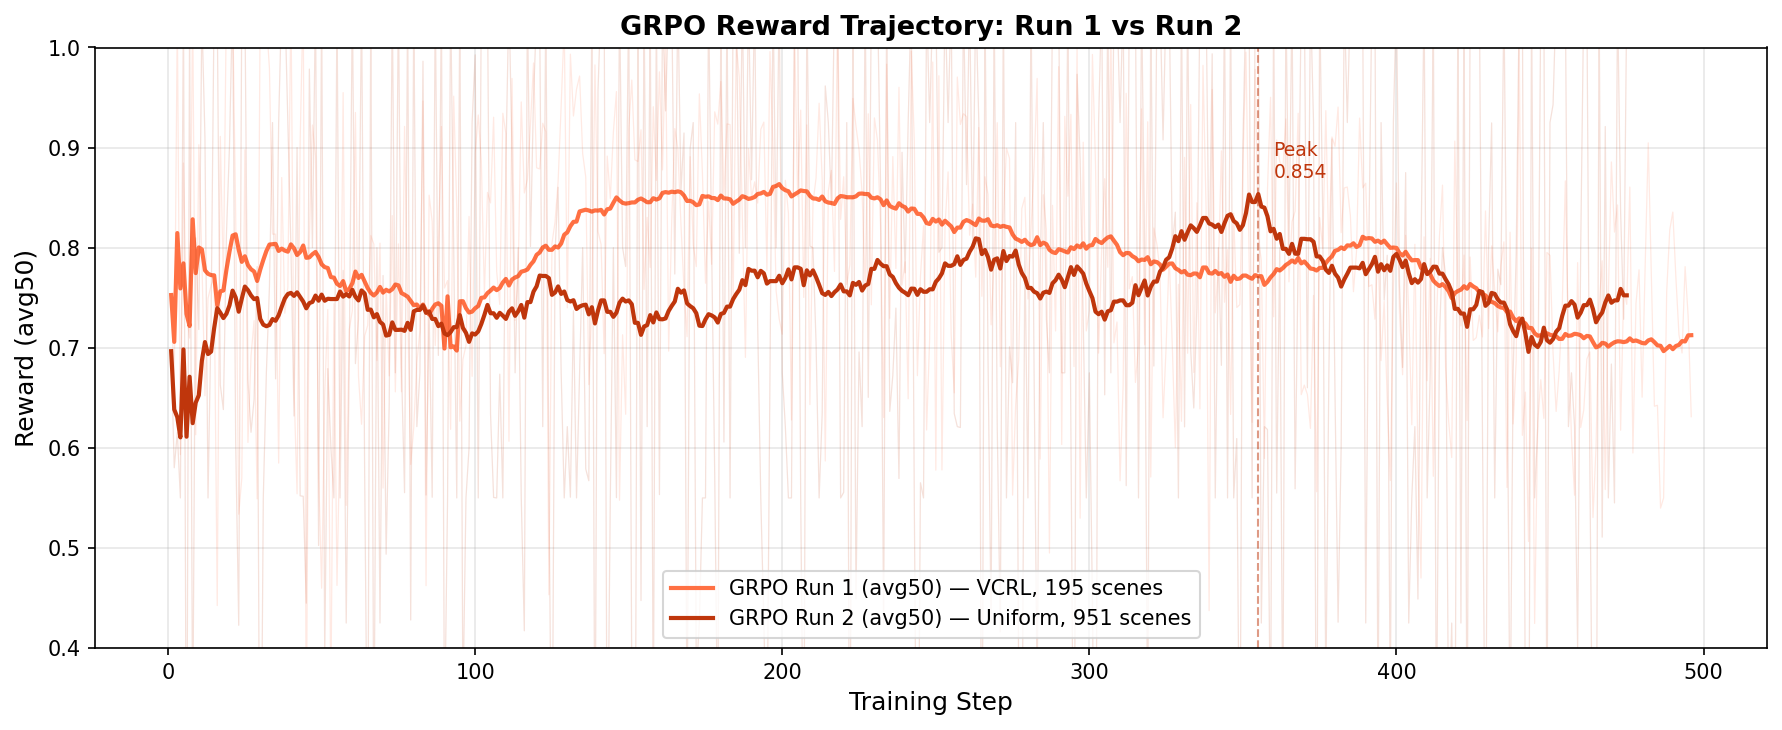
\includegraphics[width=\linewidth]{figures/grpo_reward_trajectory.png}
\caption{GRPO R3 mean reward per step (raw and 50-step EMA), compared
to the earlier Run~2 trace on uncorrected data. The corrected curriculum stays
above the Run~2 baseline throughout training; the variance reduction
visible after step $\sim$150 corresponds to the model converging on a
short MCQ-letter answer style for the categorical sub-batch.}
\label{fig:grpo_reward}
\end{figure}

\begin{figure}[h]
\centering
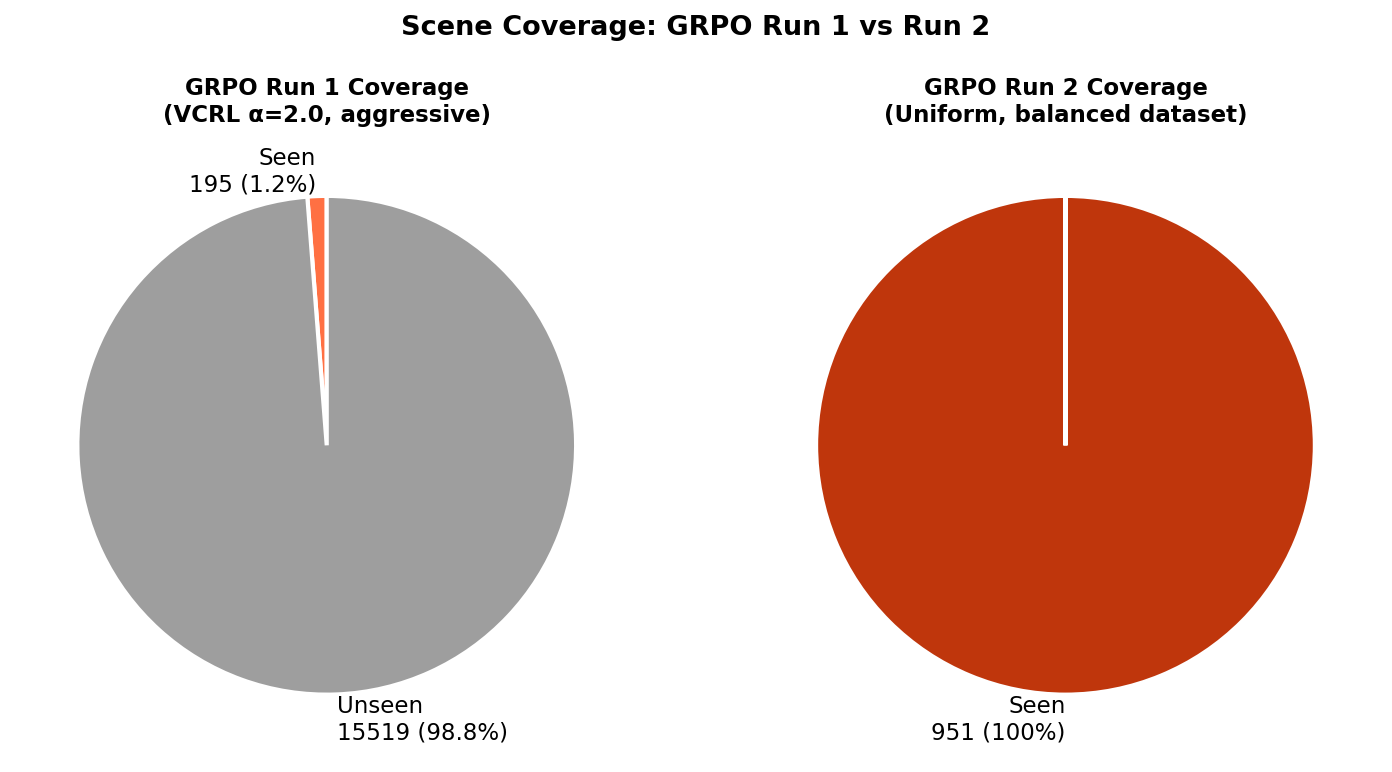
\includegraphics[width=\linewidth]{figures/grpo_coverage_comparison.png}
\caption{Per-task data coverage (fraction of GRPO rollouts per task family)
in Run~2 vs.\ R3. Run~2 was approximately $100\%$ video, leaving image-only
modes uncovered; R3 reweights to a sizeable fraction of static-image
scenes ($300/1{,}200$) plus balanced video tasks, mirroring the
corresponding PhysBench mode mix.}
\label{fig:grpo_coverage}
\end{figure}

\section{Output-Parser Sensitivity}
\label{sec:appendix-rescue}

The standard PhysBench MCQ extractor selects the \emph{last}
standalone capital letter in the response (regex
\texttt{\textbackslash b[A-D]\textbackslash b}, last match). For
SFT outputs of the form ``\texttt{B. a small cyan ball}'' the
trailing ``\texttt{a}'' (uppercased to ``A'') is preferred over
the intended leading ``B'', producing a spurious miss. A strict
extractor that prefers a leading-position option letter, and
otherwise prefers an explicit ``\texttt{Answer: X}'' or
``\texttt{X.}'' anchor, recovers a non-trivial fraction of
correct answers without re-running the model
(Table~\ref{tab:rescue}).

\begin{table}[!t]
\caption{Output-parser rescue on PhysBench Test (full
$n{=}9{,}786$). Same model outputs, only the extractor differs.}
\label{tab:rescue}
\centering
\small
\begin{tabular}{lccc}
\toprule
Checkpoint  & Standard & Strict & $\Delta$ \\
\midrule
Baseline    & 40.71 & 20.92 & $-19.79$ \\
SFT R1      & 47.51 & \textbf{48.24} & $+0.74$ \\
SFT R2-redo & 47.64 & \textbf{48.88} & $+1.24$ \\
GRPO R3     & 47.72 & 47.66 & $-0.06$ \\
\bottomrule
\end{tabular}
\end{table}

The strict extractor is not a universally better scorer:
on the baseline it discards last-letter answers the model
accidentally produces in the right position. On the SFT
checkpoints, the model emits a leading option letter often
enough that the strict extractor recovers approximately
$0.7$--$1.2$pp. GRPO R3 remains nearly flat ($-0.06$pp),
consistent with its slight response-length re-expansion
(Table~\ref{tab:cot}).

\section{Dataset Samples}
\label{sec:appendix-samples}

We show representative scenes from each of the eight training-task
families (Figs.~\ref{fig:mujoco_grid}--\ref{fig:compare_grid}) and
the heterogeneous in-the-wild PhysBench Test imagery used for
evaluation (Fig.~\ref{fig:physbench_grid}).

\begin{figure}[!t]
\centering
\setlength{\tabcolsep}{1pt}
\renewcommand{\arraystretch}{0.5}
\begin{tabular}{ccc}
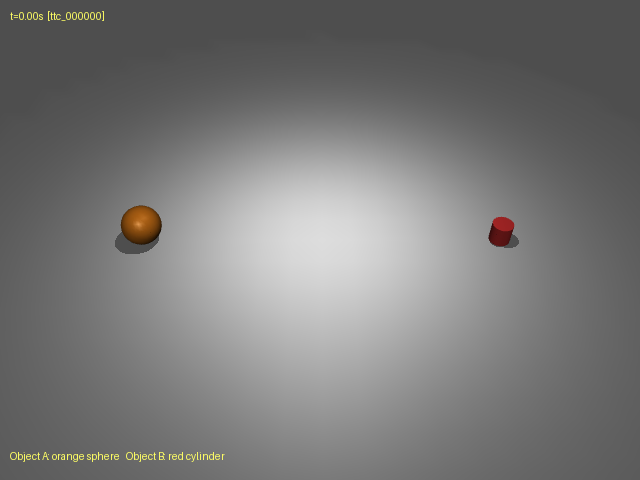
\includegraphics[width=0.30\linewidth]{samples/mujoco_ttc_frame0.png} &
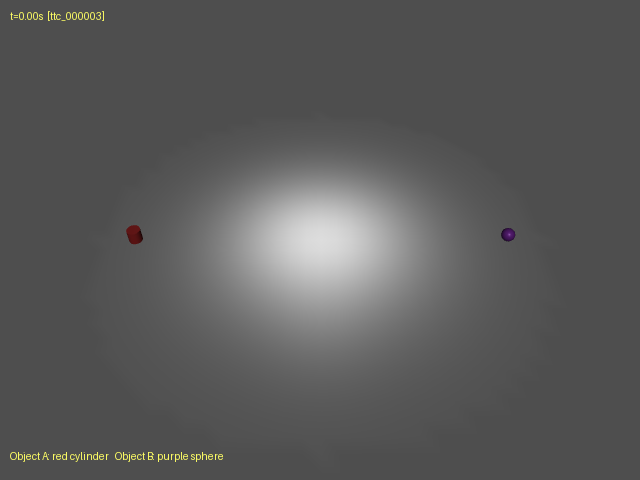
\includegraphics[width=0.30\linewidth]{samples/mujoco_ttc2_frame0.png} &
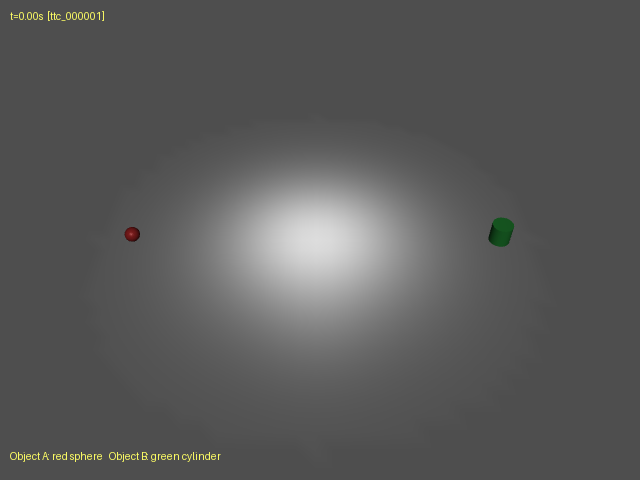
\includegraphics[width=0.30\linewidth]{samples/mujoco_ttc3_f0.png} \\
\multicolumn{3}{c}{\footnotesize (a) Time-to-collision (TTC)}\\[2pt]
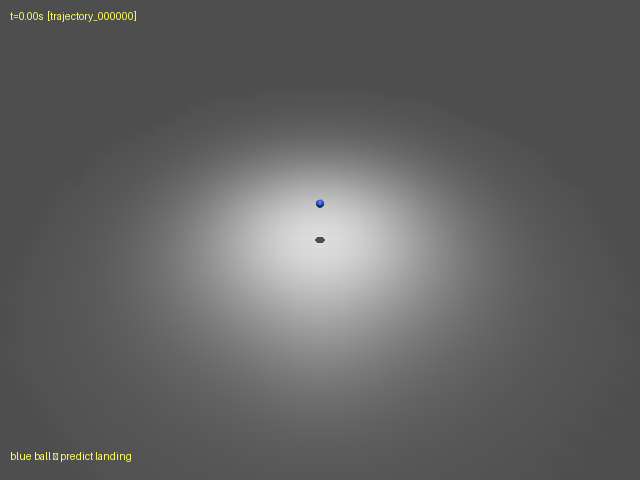
\includegraphics[width=0.30\linewidth]{samples/mujoco_trajectory_frame0.png} &
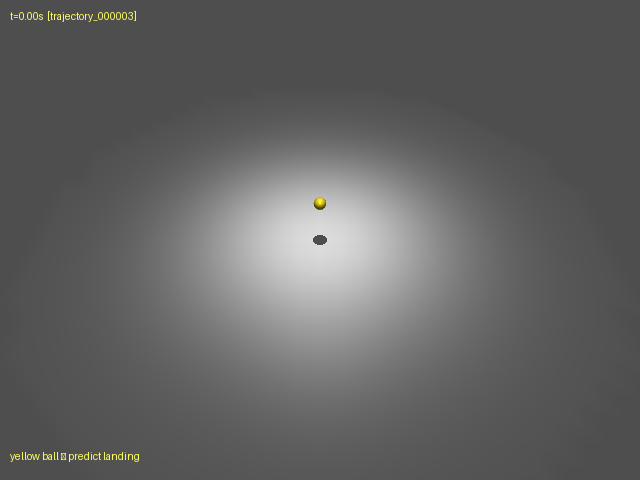
\includegraphics[width=0.30\linewidth]{samples/mujoco_trajectory2_frame0.png} &
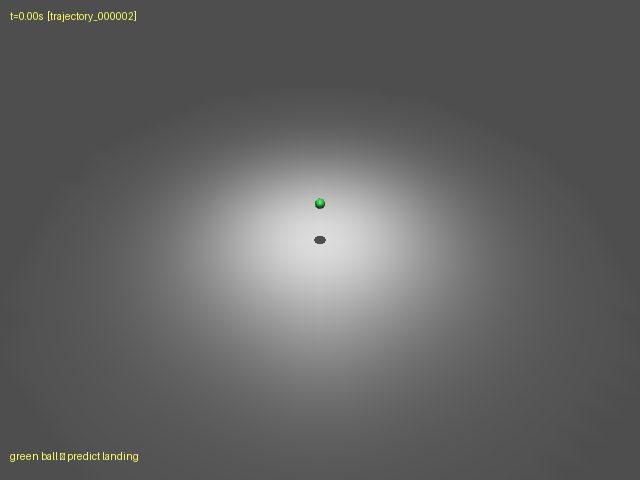
\includegraphics[width=0.30\linewidth]{samples/mujoco_traj3_f0.png} \\
\multicolumn{3}{c}{\footnotesize (b) Projectile trajectory}\\[2pt]
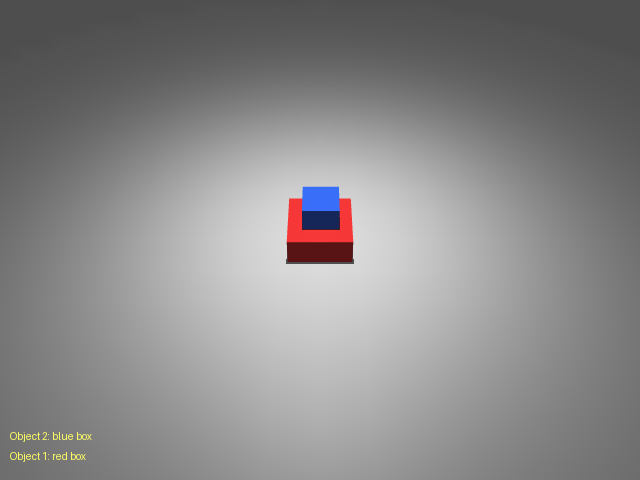
\includegraphics[width=0.30\linewidth]{samples/mujoco_stability.png} &
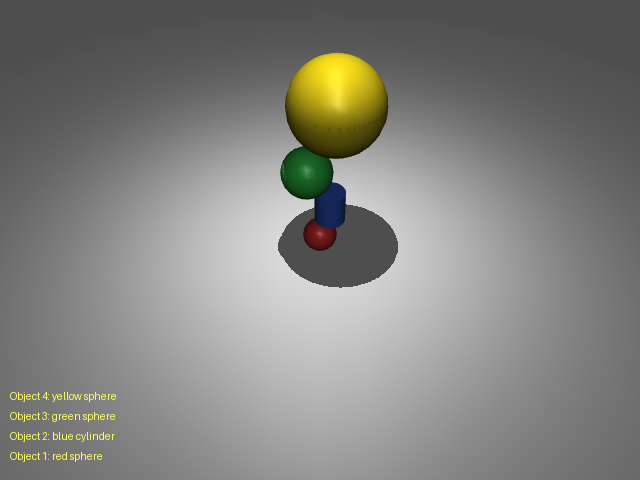
\includegraphics[width=0.30\linewidth]{samples/mujoco_stability2.png} &
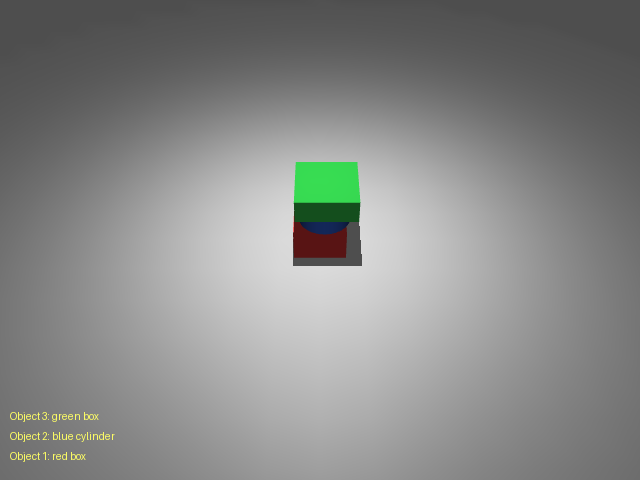
\includegraphics[width=0.30\linewidth]{samples/mujoco_stability3.png} \\
\multicolumn{3}{c}{\footnotesize (c) Pile stability}\\
\end{tabular}
\caption{MuJoCo training scenes used in SFT R1: time-to-collision,
projectile trajectory, and pile stability. Each scene is rendered as
an $8$-frame rollout; first frame shown.}
\label{fig:mujoco_grid}
\end{figure}

\begin{figure}[!t]
\centering
\setlength{\tabcolsep}{1pt}
\renewcommand{\arraystretch}{0.5}
\begin{tabular}{ccc}
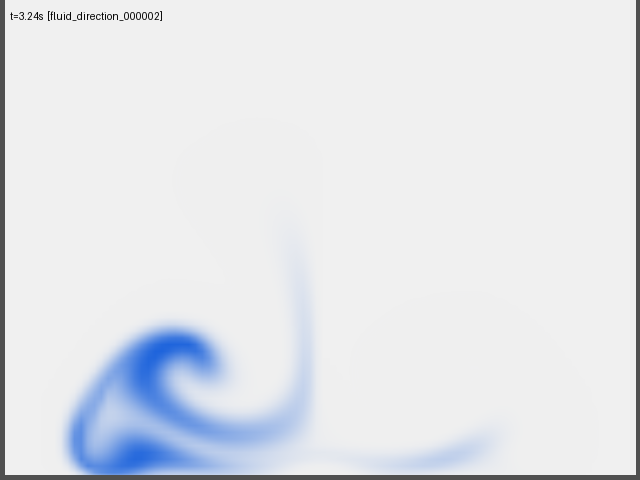
\includegraphics[width=0.30\linewidth]{samples/phiflow_corrected/dir_down.png} &
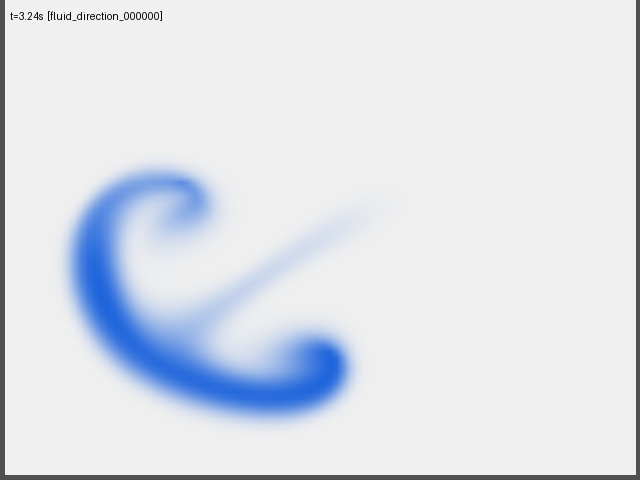
\includegraphics[width=0.30\linewidth]{samples/phiflow_corrected/dir_left.png} &
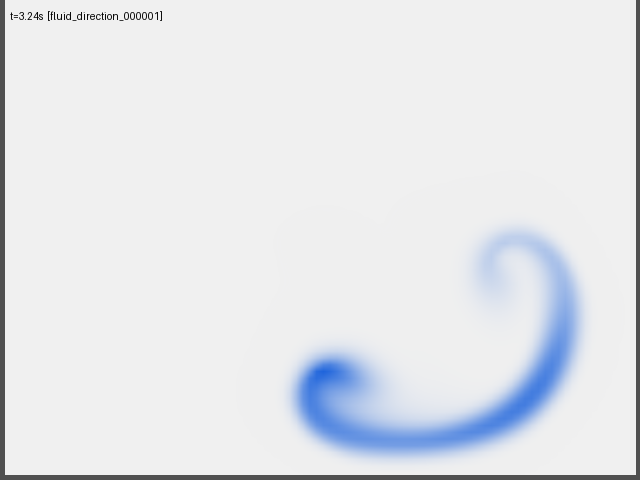
\includegraphics[width=0.30\linewidth]{samples/phiflow_corrected/dir_right.png} \\
\multicolumn{3}{c}{\footnotesize (a) Fluid direction}\\[2pt]
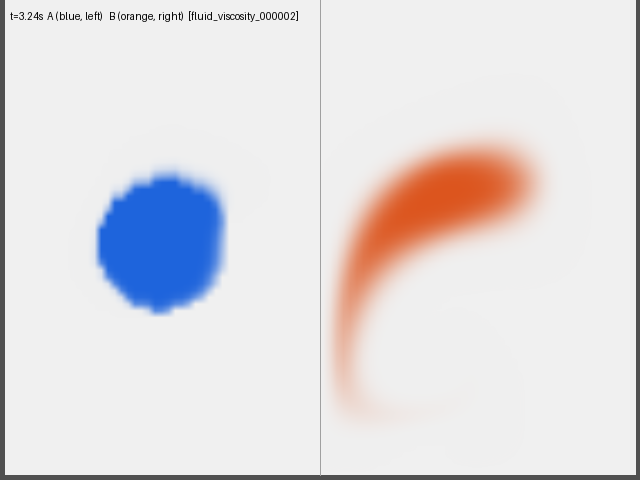
\includegraphics[width=0.30\linewidth]{samples/phiflow_corrected/visc_low.png} &
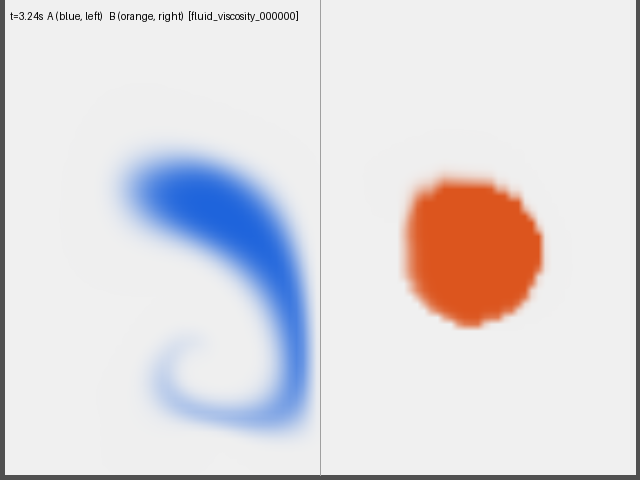
\includegraphics[width=0.30\linewidth]{samples/phiflow_corrected/visc_high.png} &
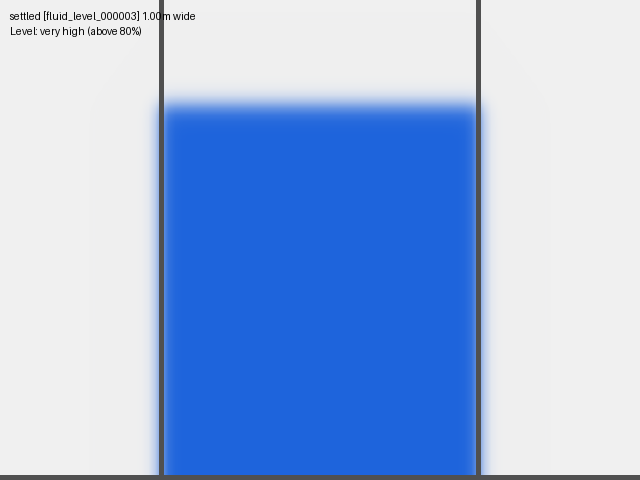
\includegraphics[width=0.30\linewidth]{samples/phiflow_corrected/level_high.png} \\
\multicolumn{3}{c}{\footnotesize (b) Viscosity (low / high) and fluid level (high)}\\
\end{tabular}
\caption{PhiFlow training scenes used in SFT R2-redo: flow direction,
viscosity comparison, and fluid level. Rendered top-down at
$256{\times}256$ via particle deposition + Gaussian density filter
($\sigma=7$ px).}
\label{fig:phiflow_grid}
\end{figure}

\begin{figure}[!t]
\centering
\setlength{\tabcolsep}{1pt}
\renewcommand{\arraystretch}{0.5}
\begin{tabular}{ccc}
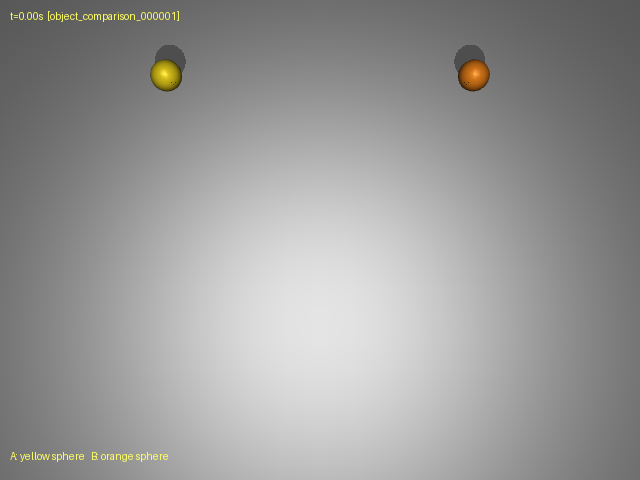
\includegraphics[width=0.30\linewidth]{samples/object_comparison_heavier_f0.png} &
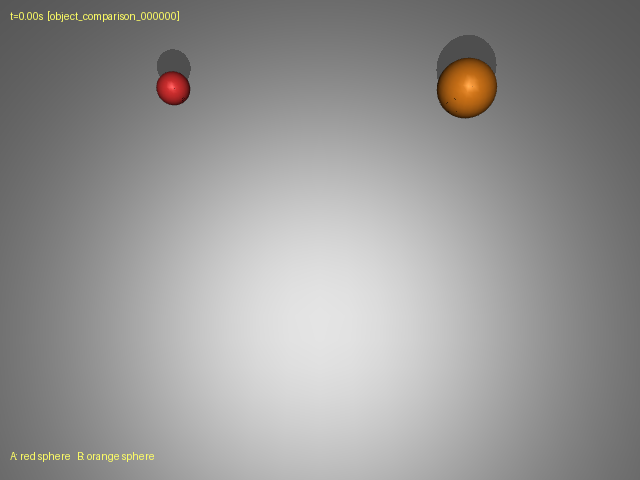
\includegraphics[width=0.30\linewidth]{samples/object_comparison_larger_f0.png} &
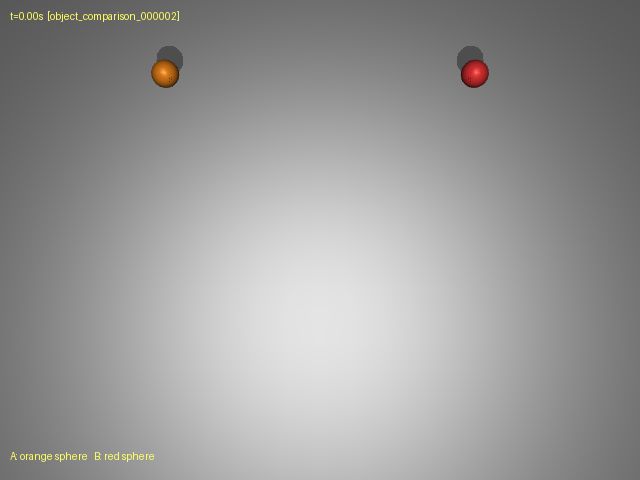
\includegraphics[width=0.30\linewidth]{samples/object_comparison_bouncier_f0.png} \\
\multicolumn{3}{c}{\footnotesize (a) Object comparisons: heavier, larger, bouncier}\\[2pt]
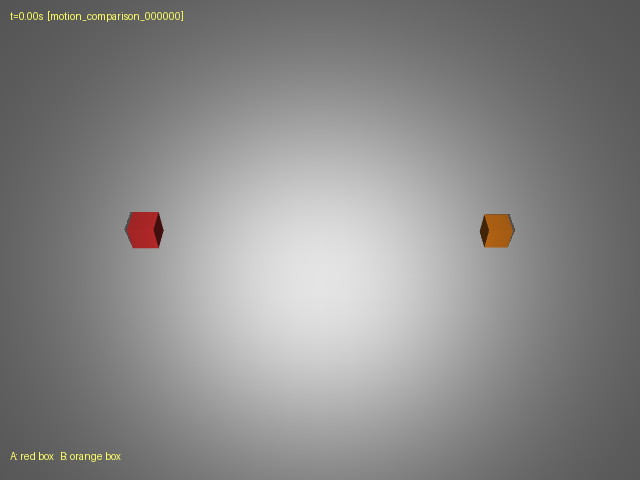
\includegraphics[width=0.30\linewidth]{samples/motion_comparison_faster_f0.png} &
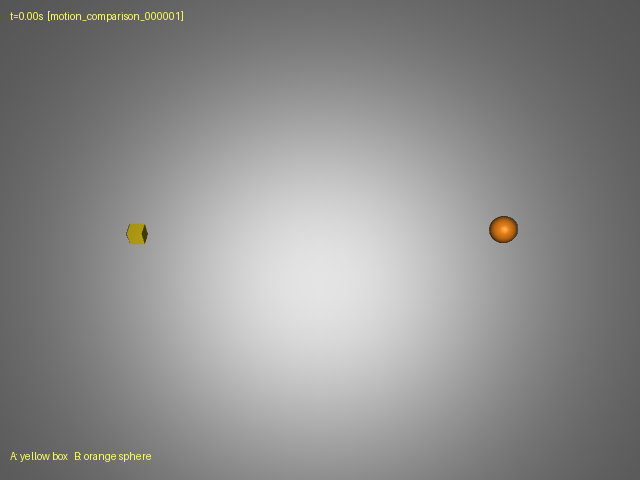
\includegraphics[width=0.30\linewidth]{samples/motion_comparison_higher_f0.png} &
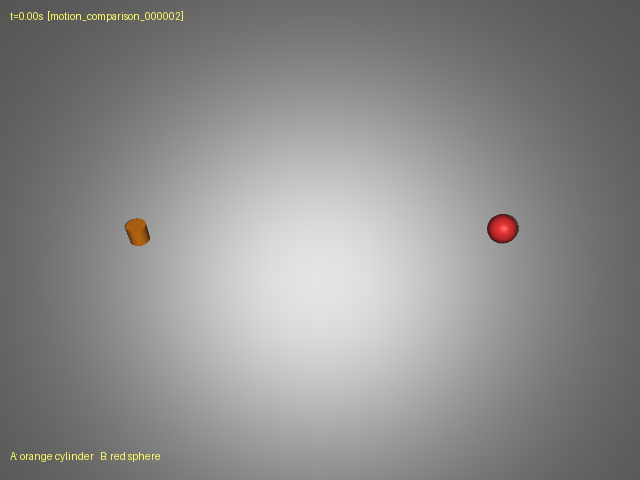
\includegraphics[width=0.30\linewidth]{samples/motion_comparison_farther_f0.png} \\
\multicolumn{3}{c}{\footnotesize (b) Motion comparisons: faster, higher, farther}\\
\end{tabular}
\caption{Categorical comparison scenes used in SFT R2-redo (object
mass/size/elasticity and motion magnitude). The model is asked to
identify the correct object from a short free-text answer
(e.g.\ \texttt{<answer>red</answer>}); ground truth is read directly
from the simulator state.}
\label{fig:compare_grid}
\end{figure}

\begin{figure}[!t]
\centering
\setlength{\tabcolsep}{1pt}
\renewcommand{\arraystretch}{0.5}
\begin{tabular}{cccc}
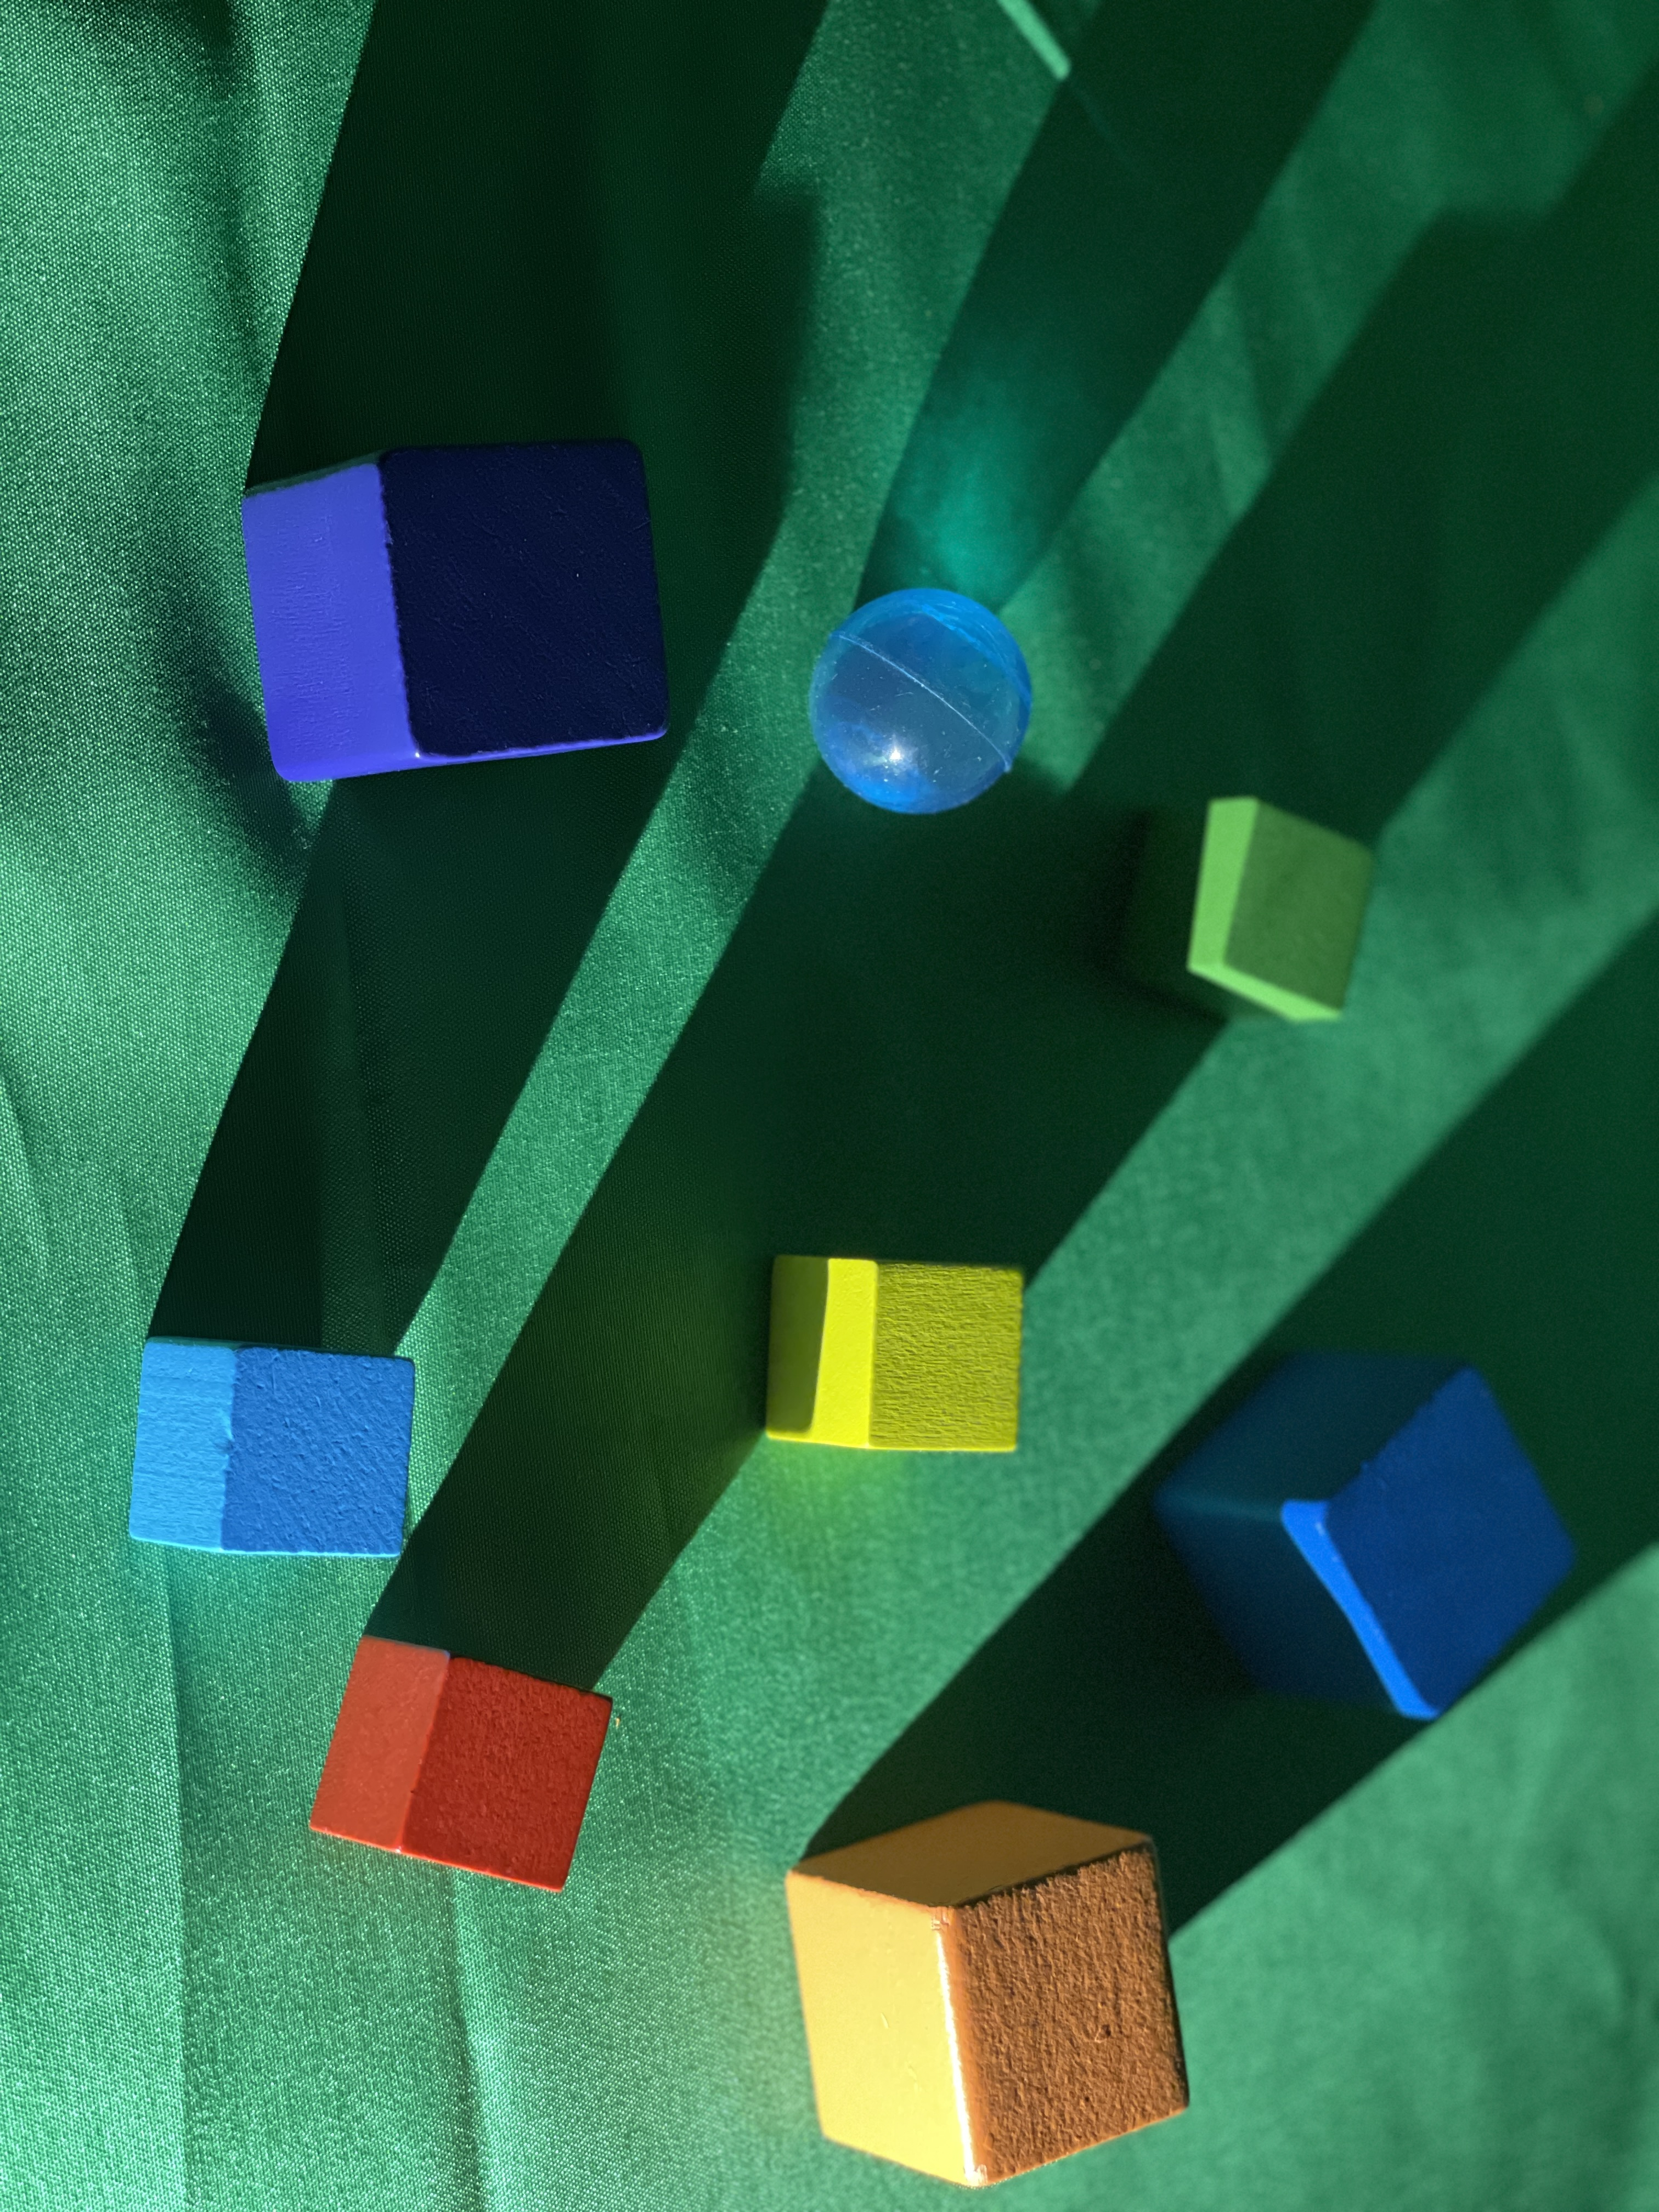
\includegraphics[width=0.22\linewidth]{samples/pb_property_attribute_image_only.JPG} &
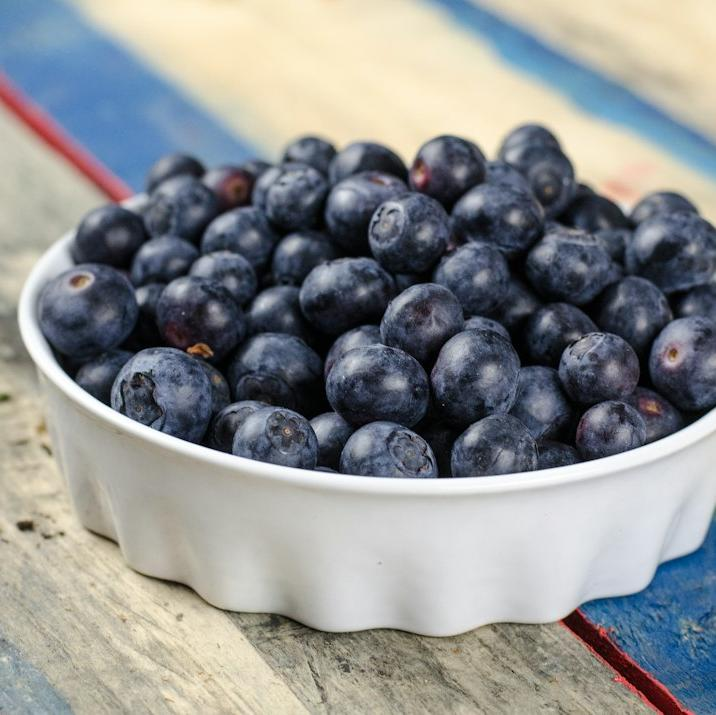
\includegraphics[width=0.22\linewidth]{samples/pb_property_color_image_only.jpg} &
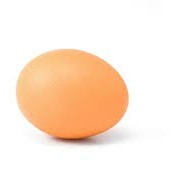
\includegraphics[width=0.22\linewidth]{samples/pb_property_mass_image_only.jpg} &
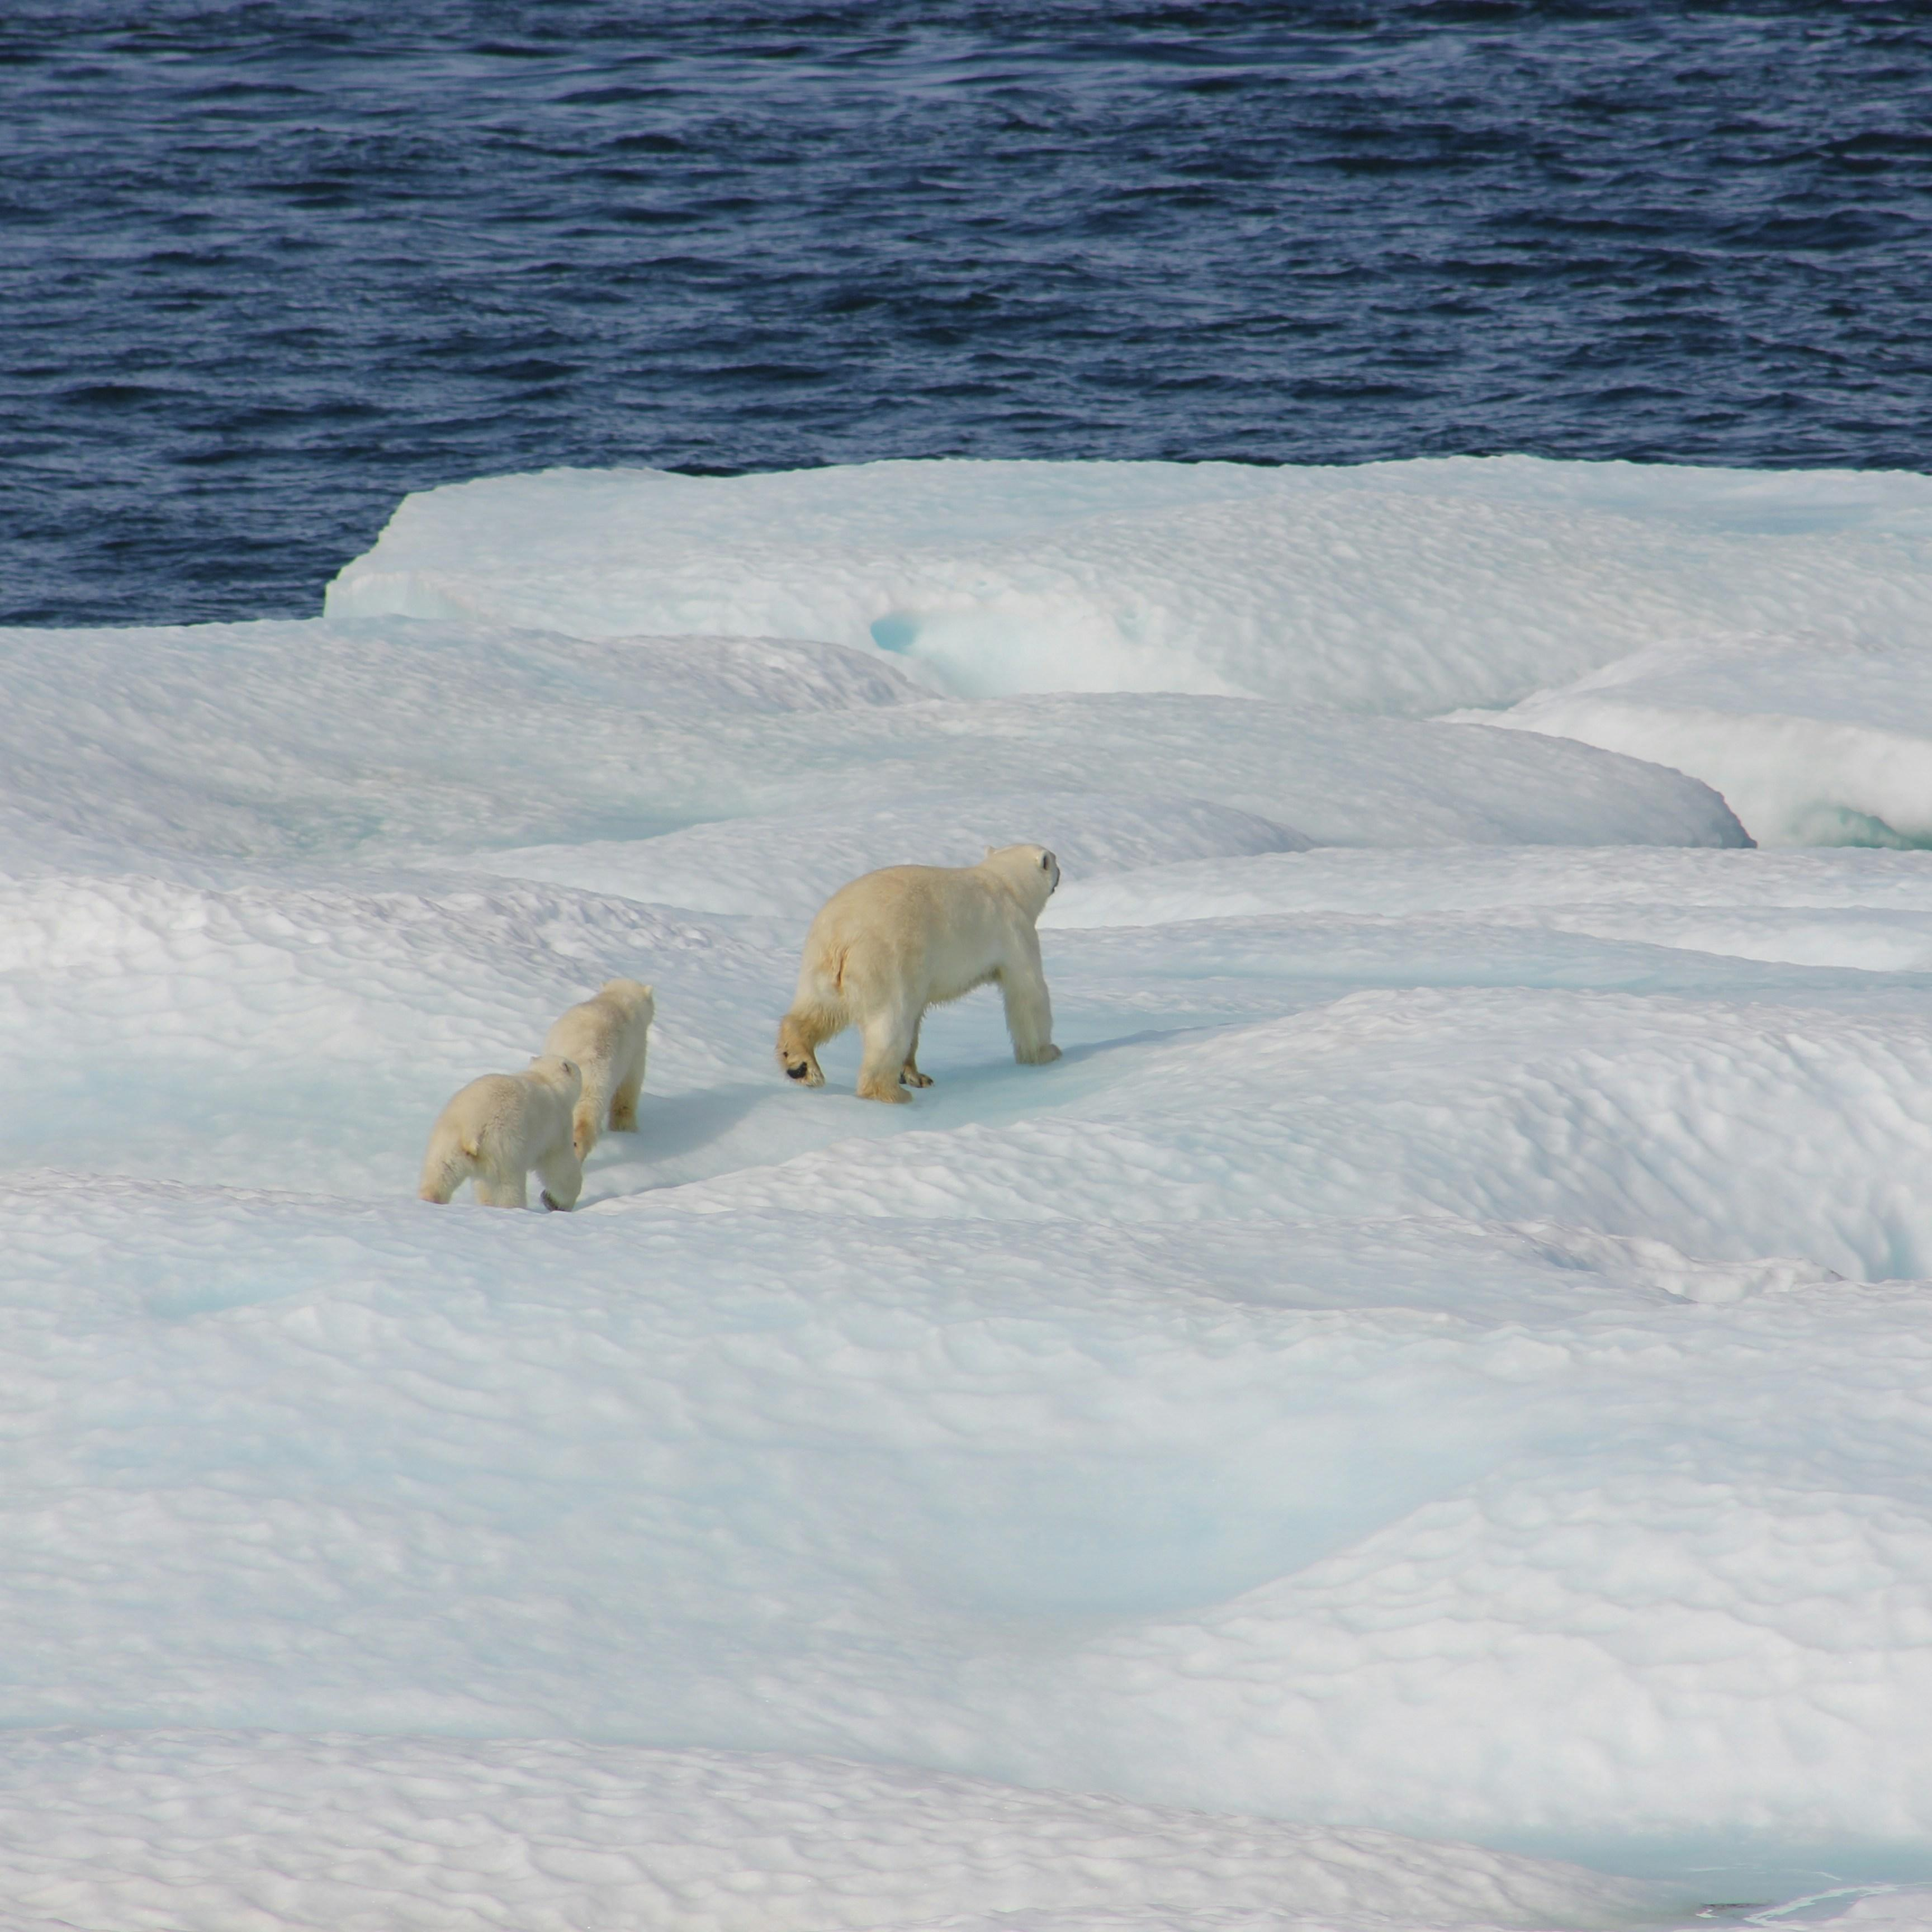
\includegraphics[width=0.22\linewidth]{samples/pb_property_number_image_only.jpg} \\
\multicolumn{4}{c}{\footnotesize (a) \textbf{Property}: attribute, colour, mass, number}\\[2pt]
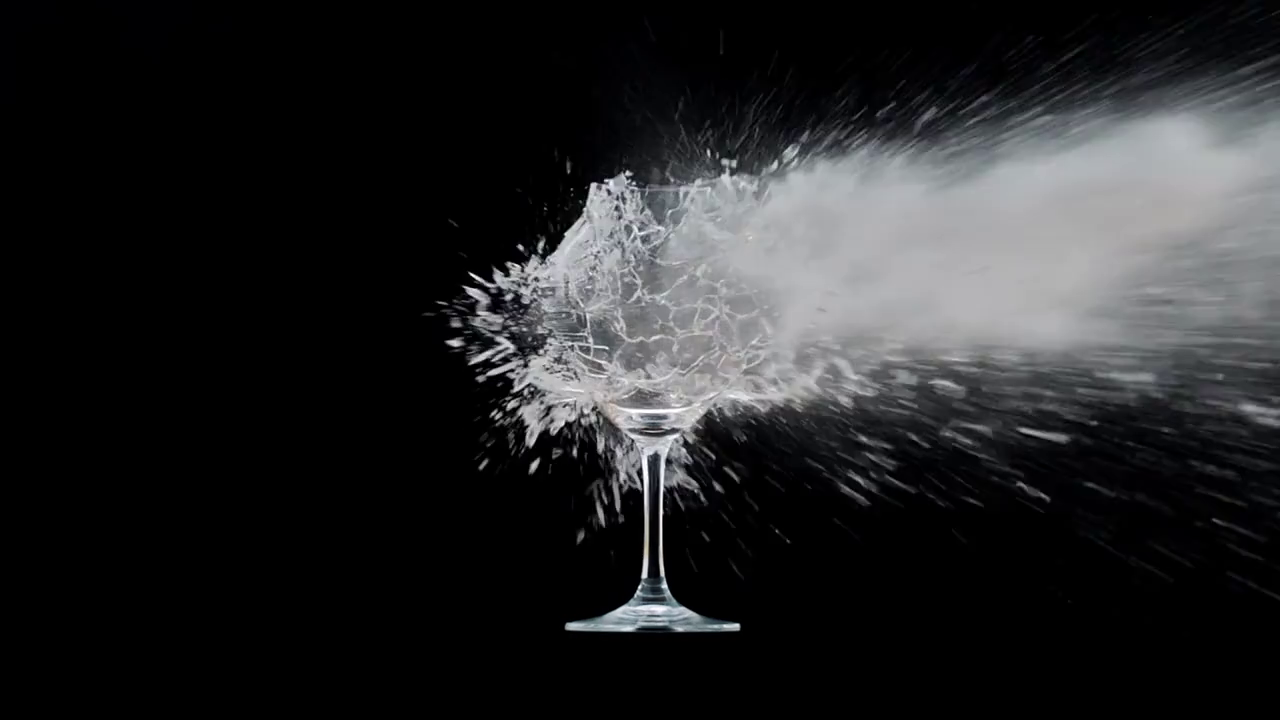
\includegraphics[width=0.22\linewidth]{samples/pb_dynamics_collision_image_only.png} &
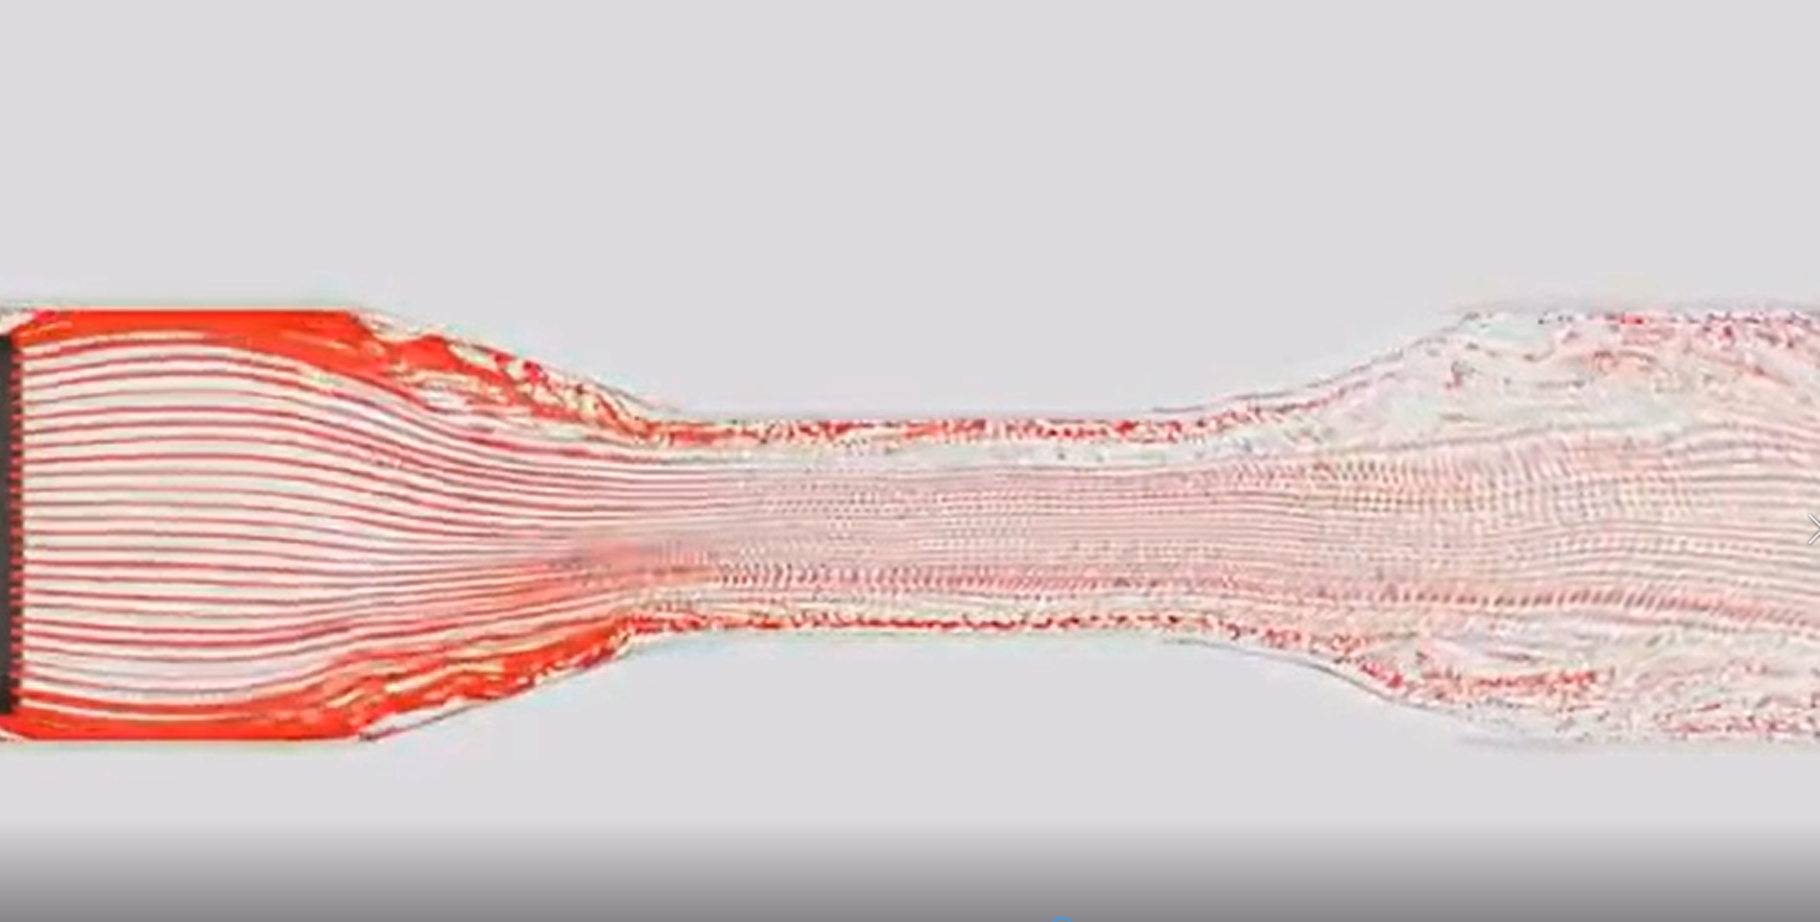
\includegraphics[width=0.22\linewidth]{samples/pb_dynamics_fluid_image_only.png} &
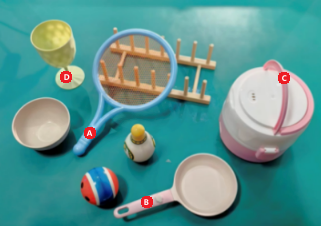
\includegraphics[width=0.22\linewidth]{samples/pb_dynamics_manipulation_image_only.png} &
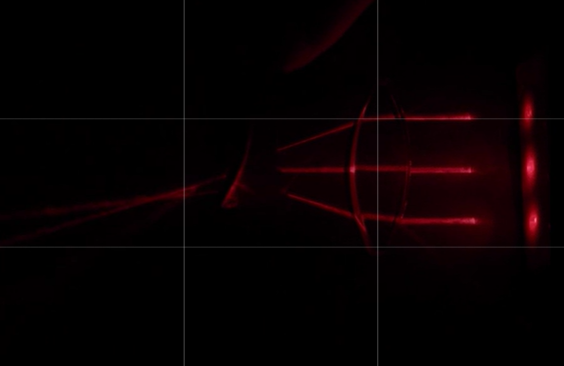
\includegraphics[width=0.22\linewidth]{samples/pb_dynamics_others_general.png} \\
\multicolumn{4}{c}{\footnotesize (b) \textbf{Dynamics}: collision, fluid, manipulation, others}\\[2pt]
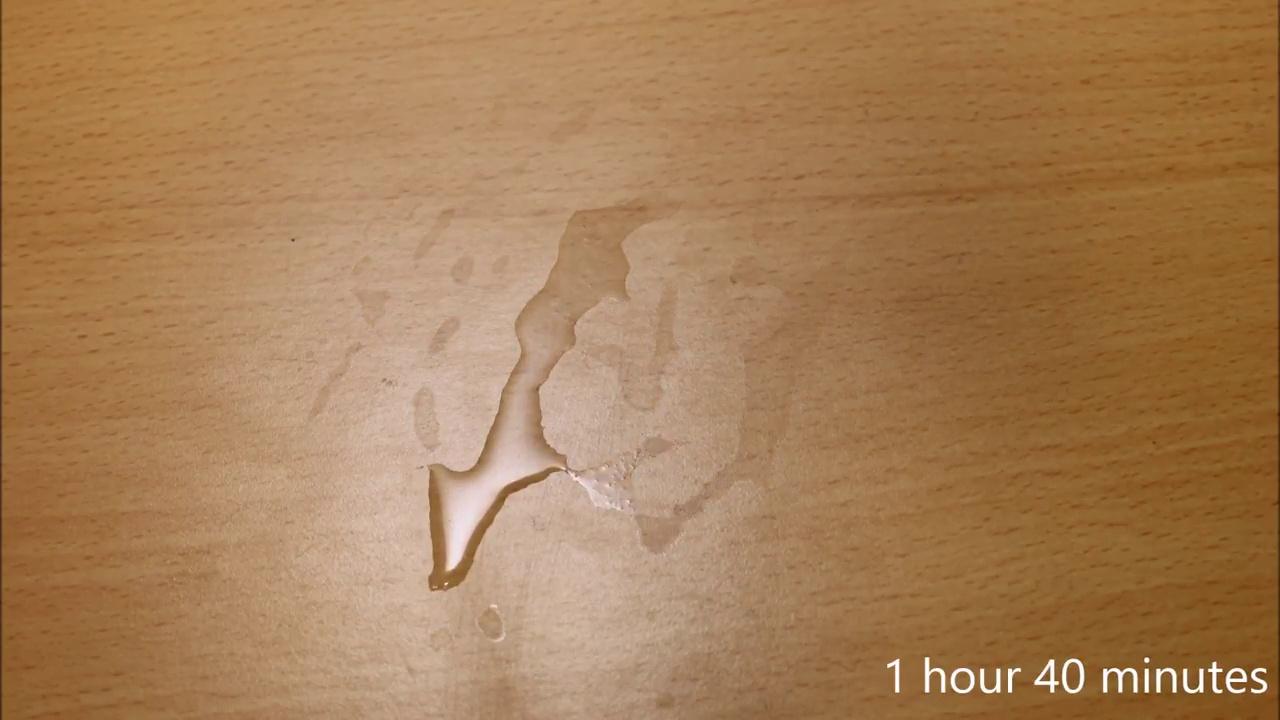
\includegraphics[width=0.22\linewidth]{samples/pb_scene_air_general.jpg} &
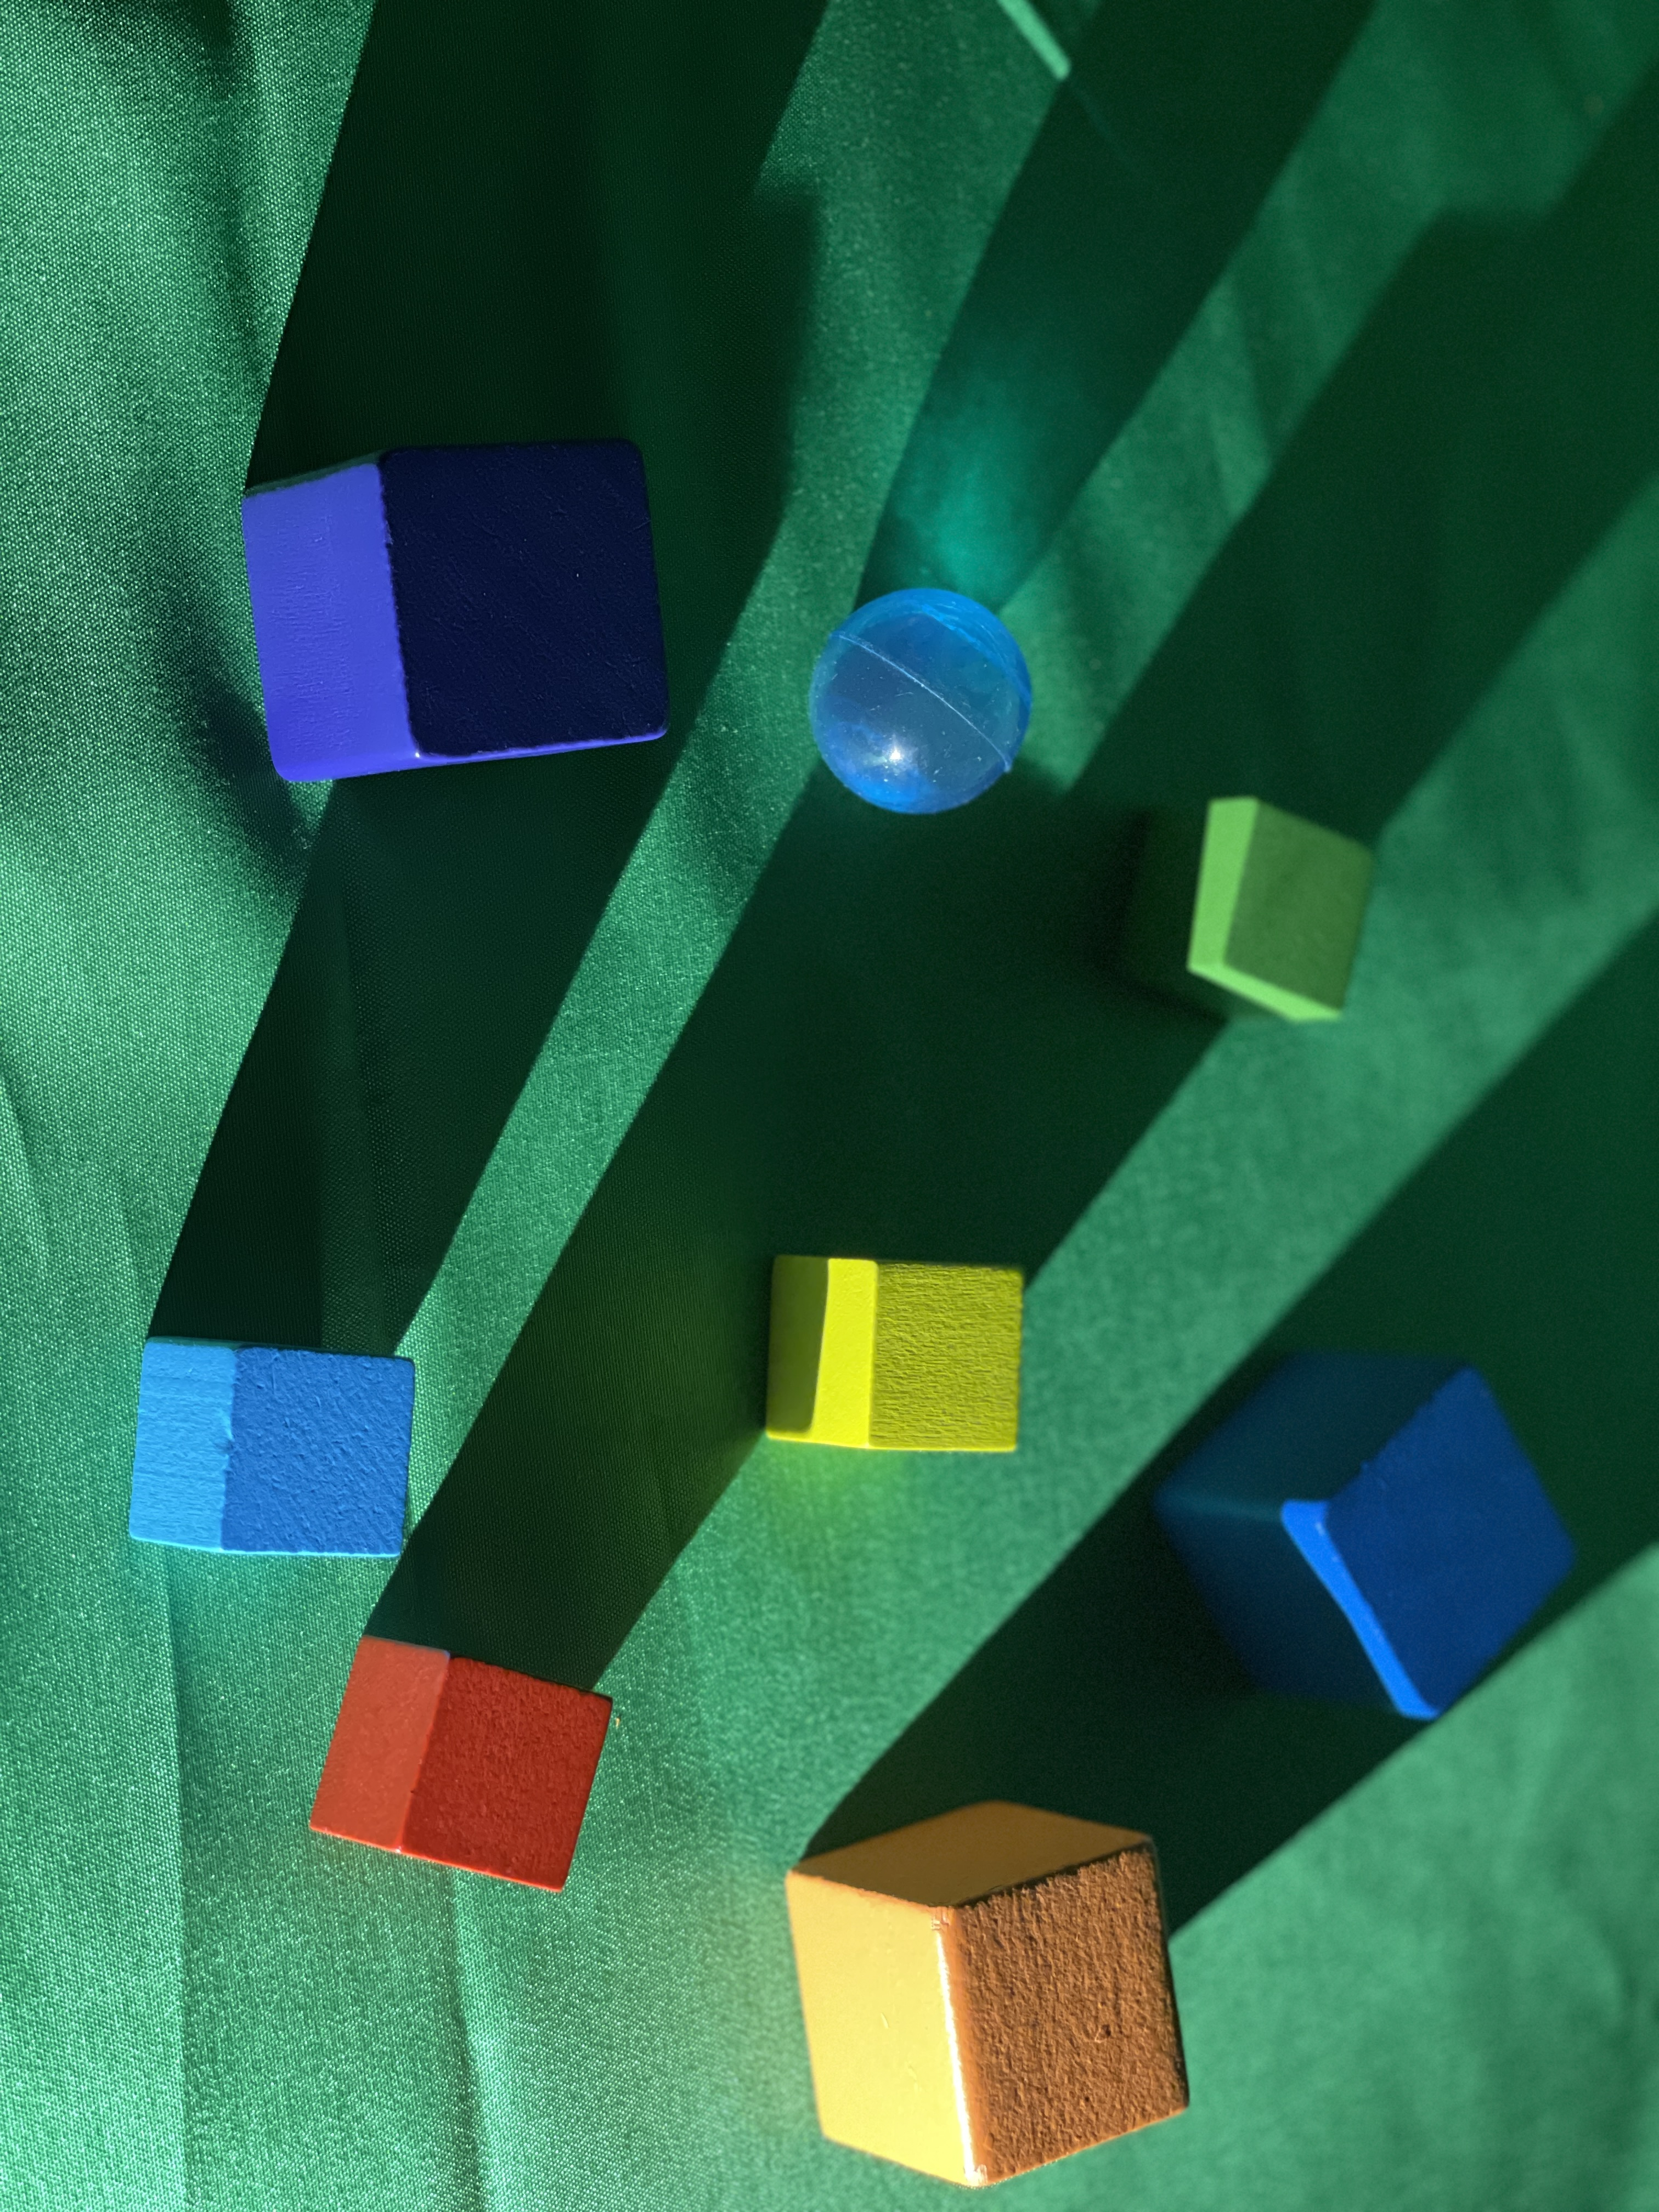
\includegraphics[width=0.22\linewidth]{samples/pb_scene_light_image_only.JPG} &
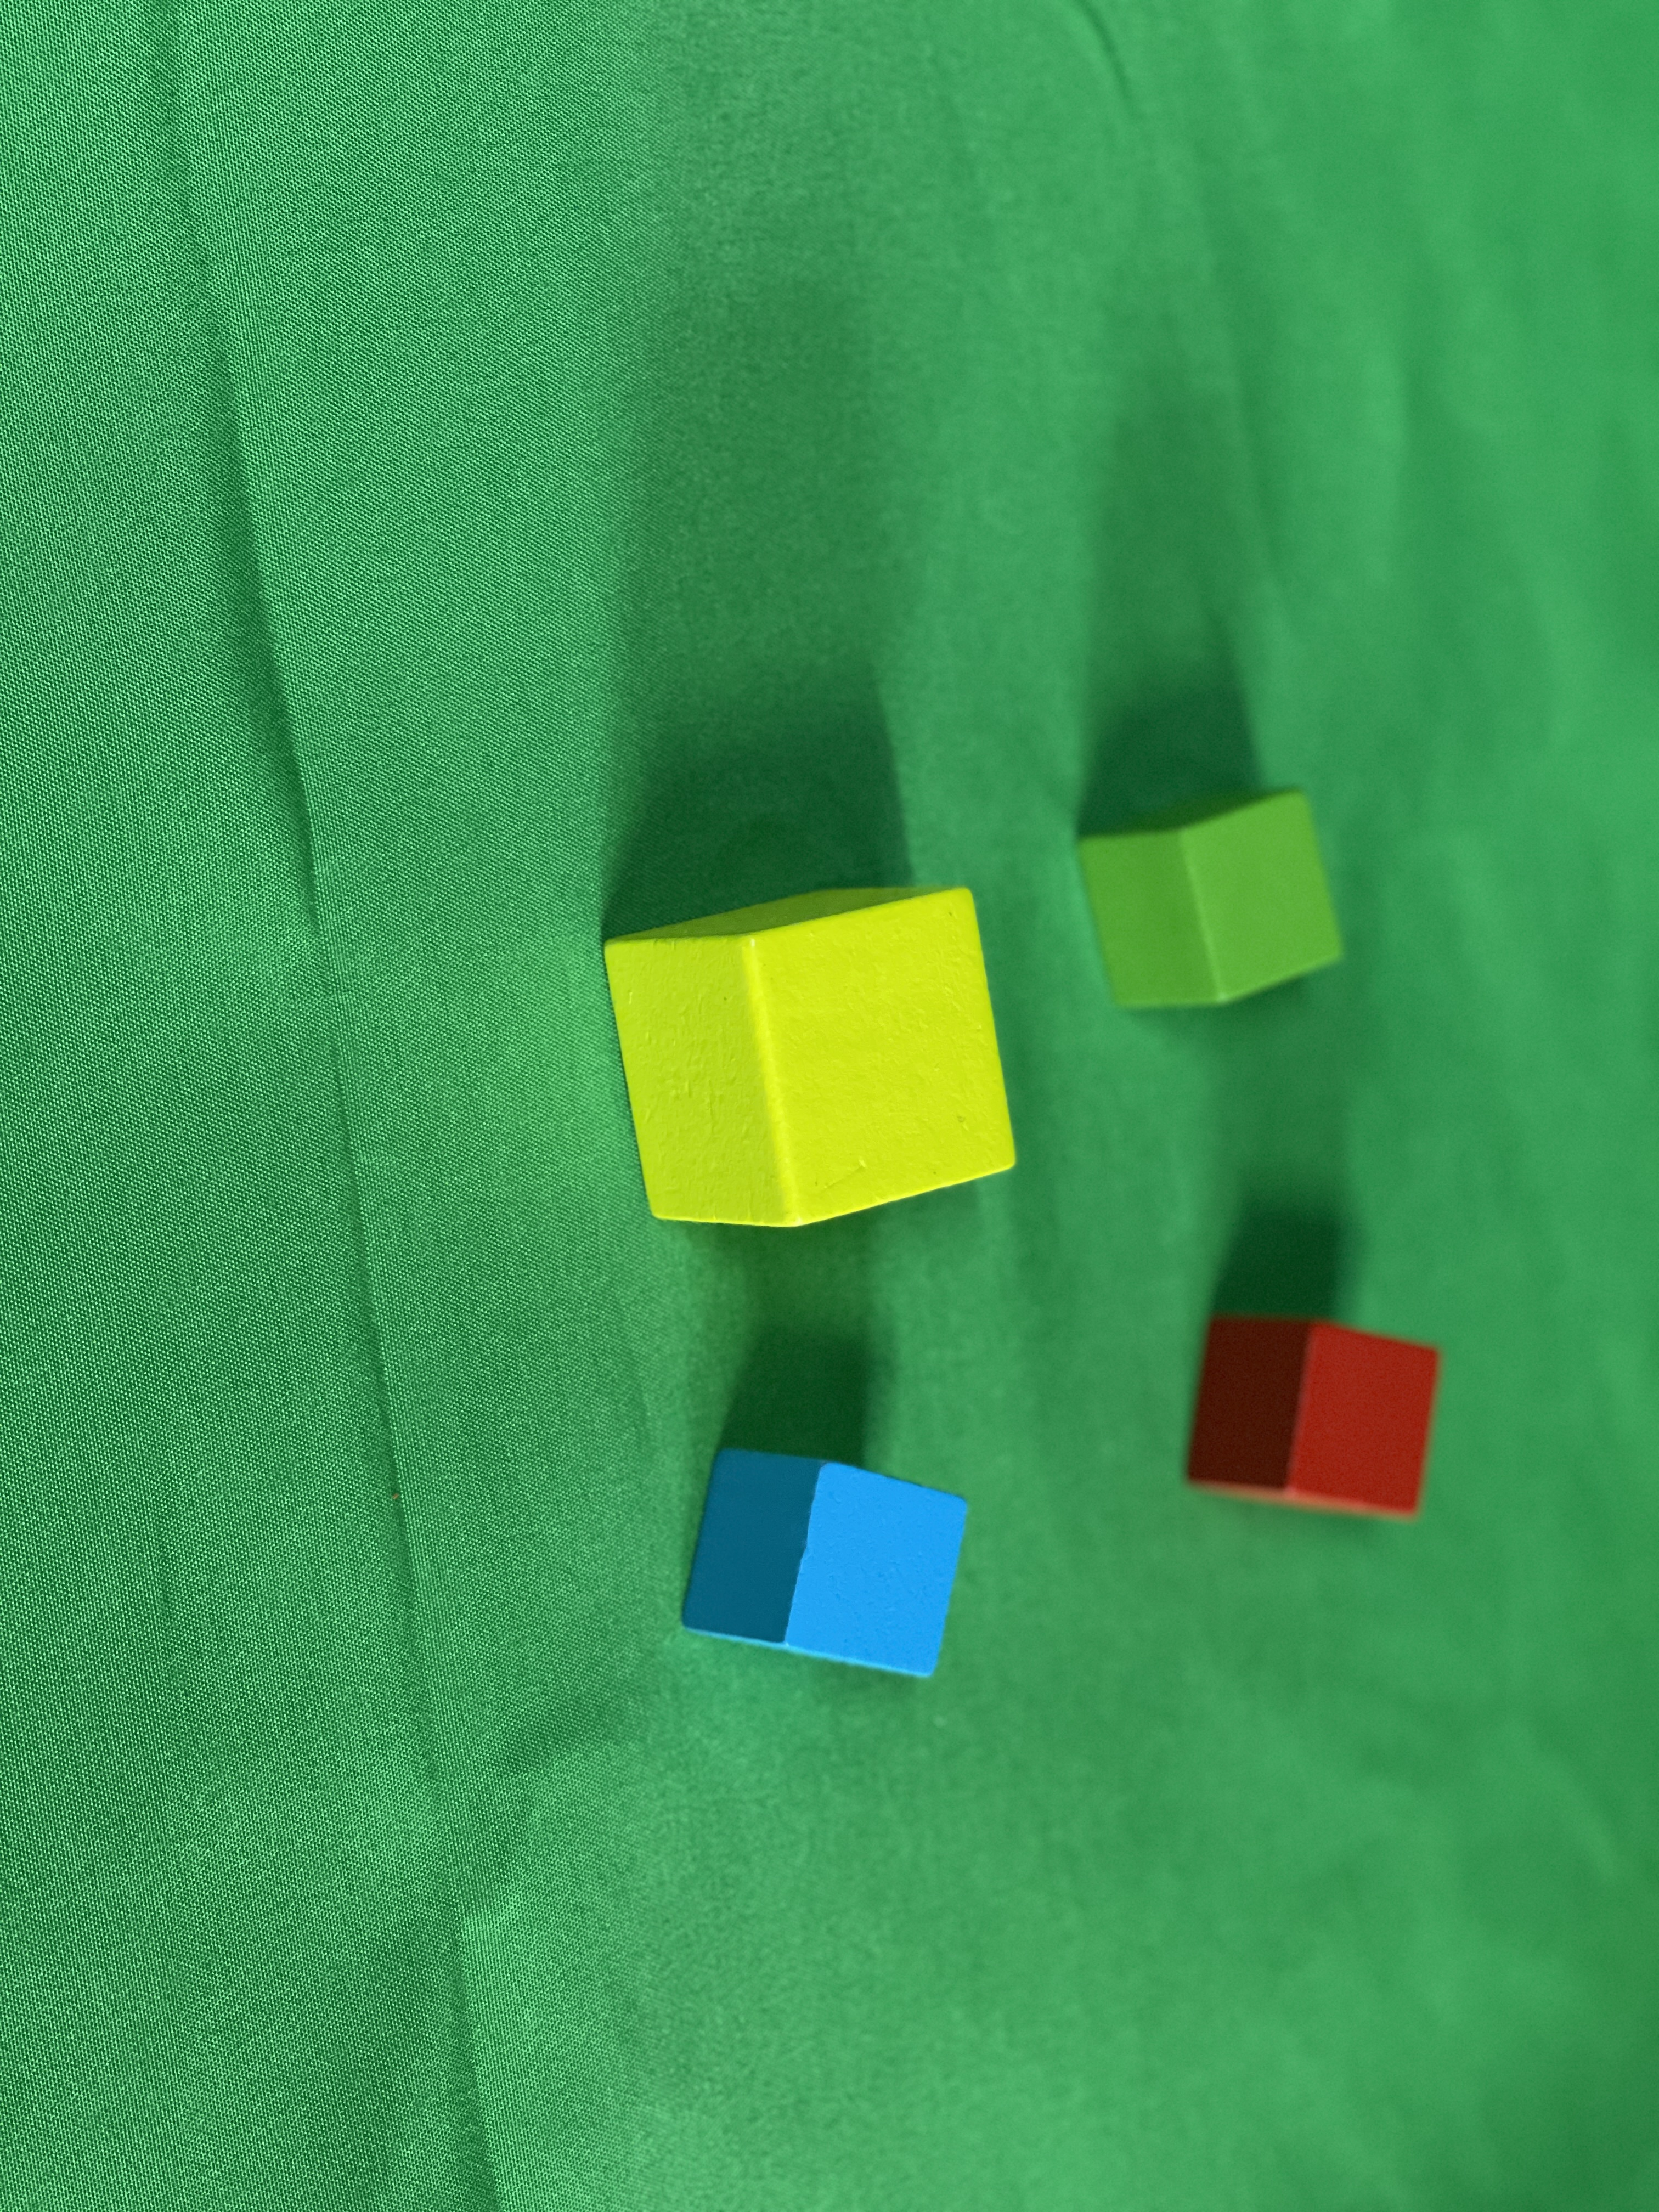
\includegraphics[width=0.22\linewidth]{samples/pb_scene_viewpoint_image_only.JPG} &
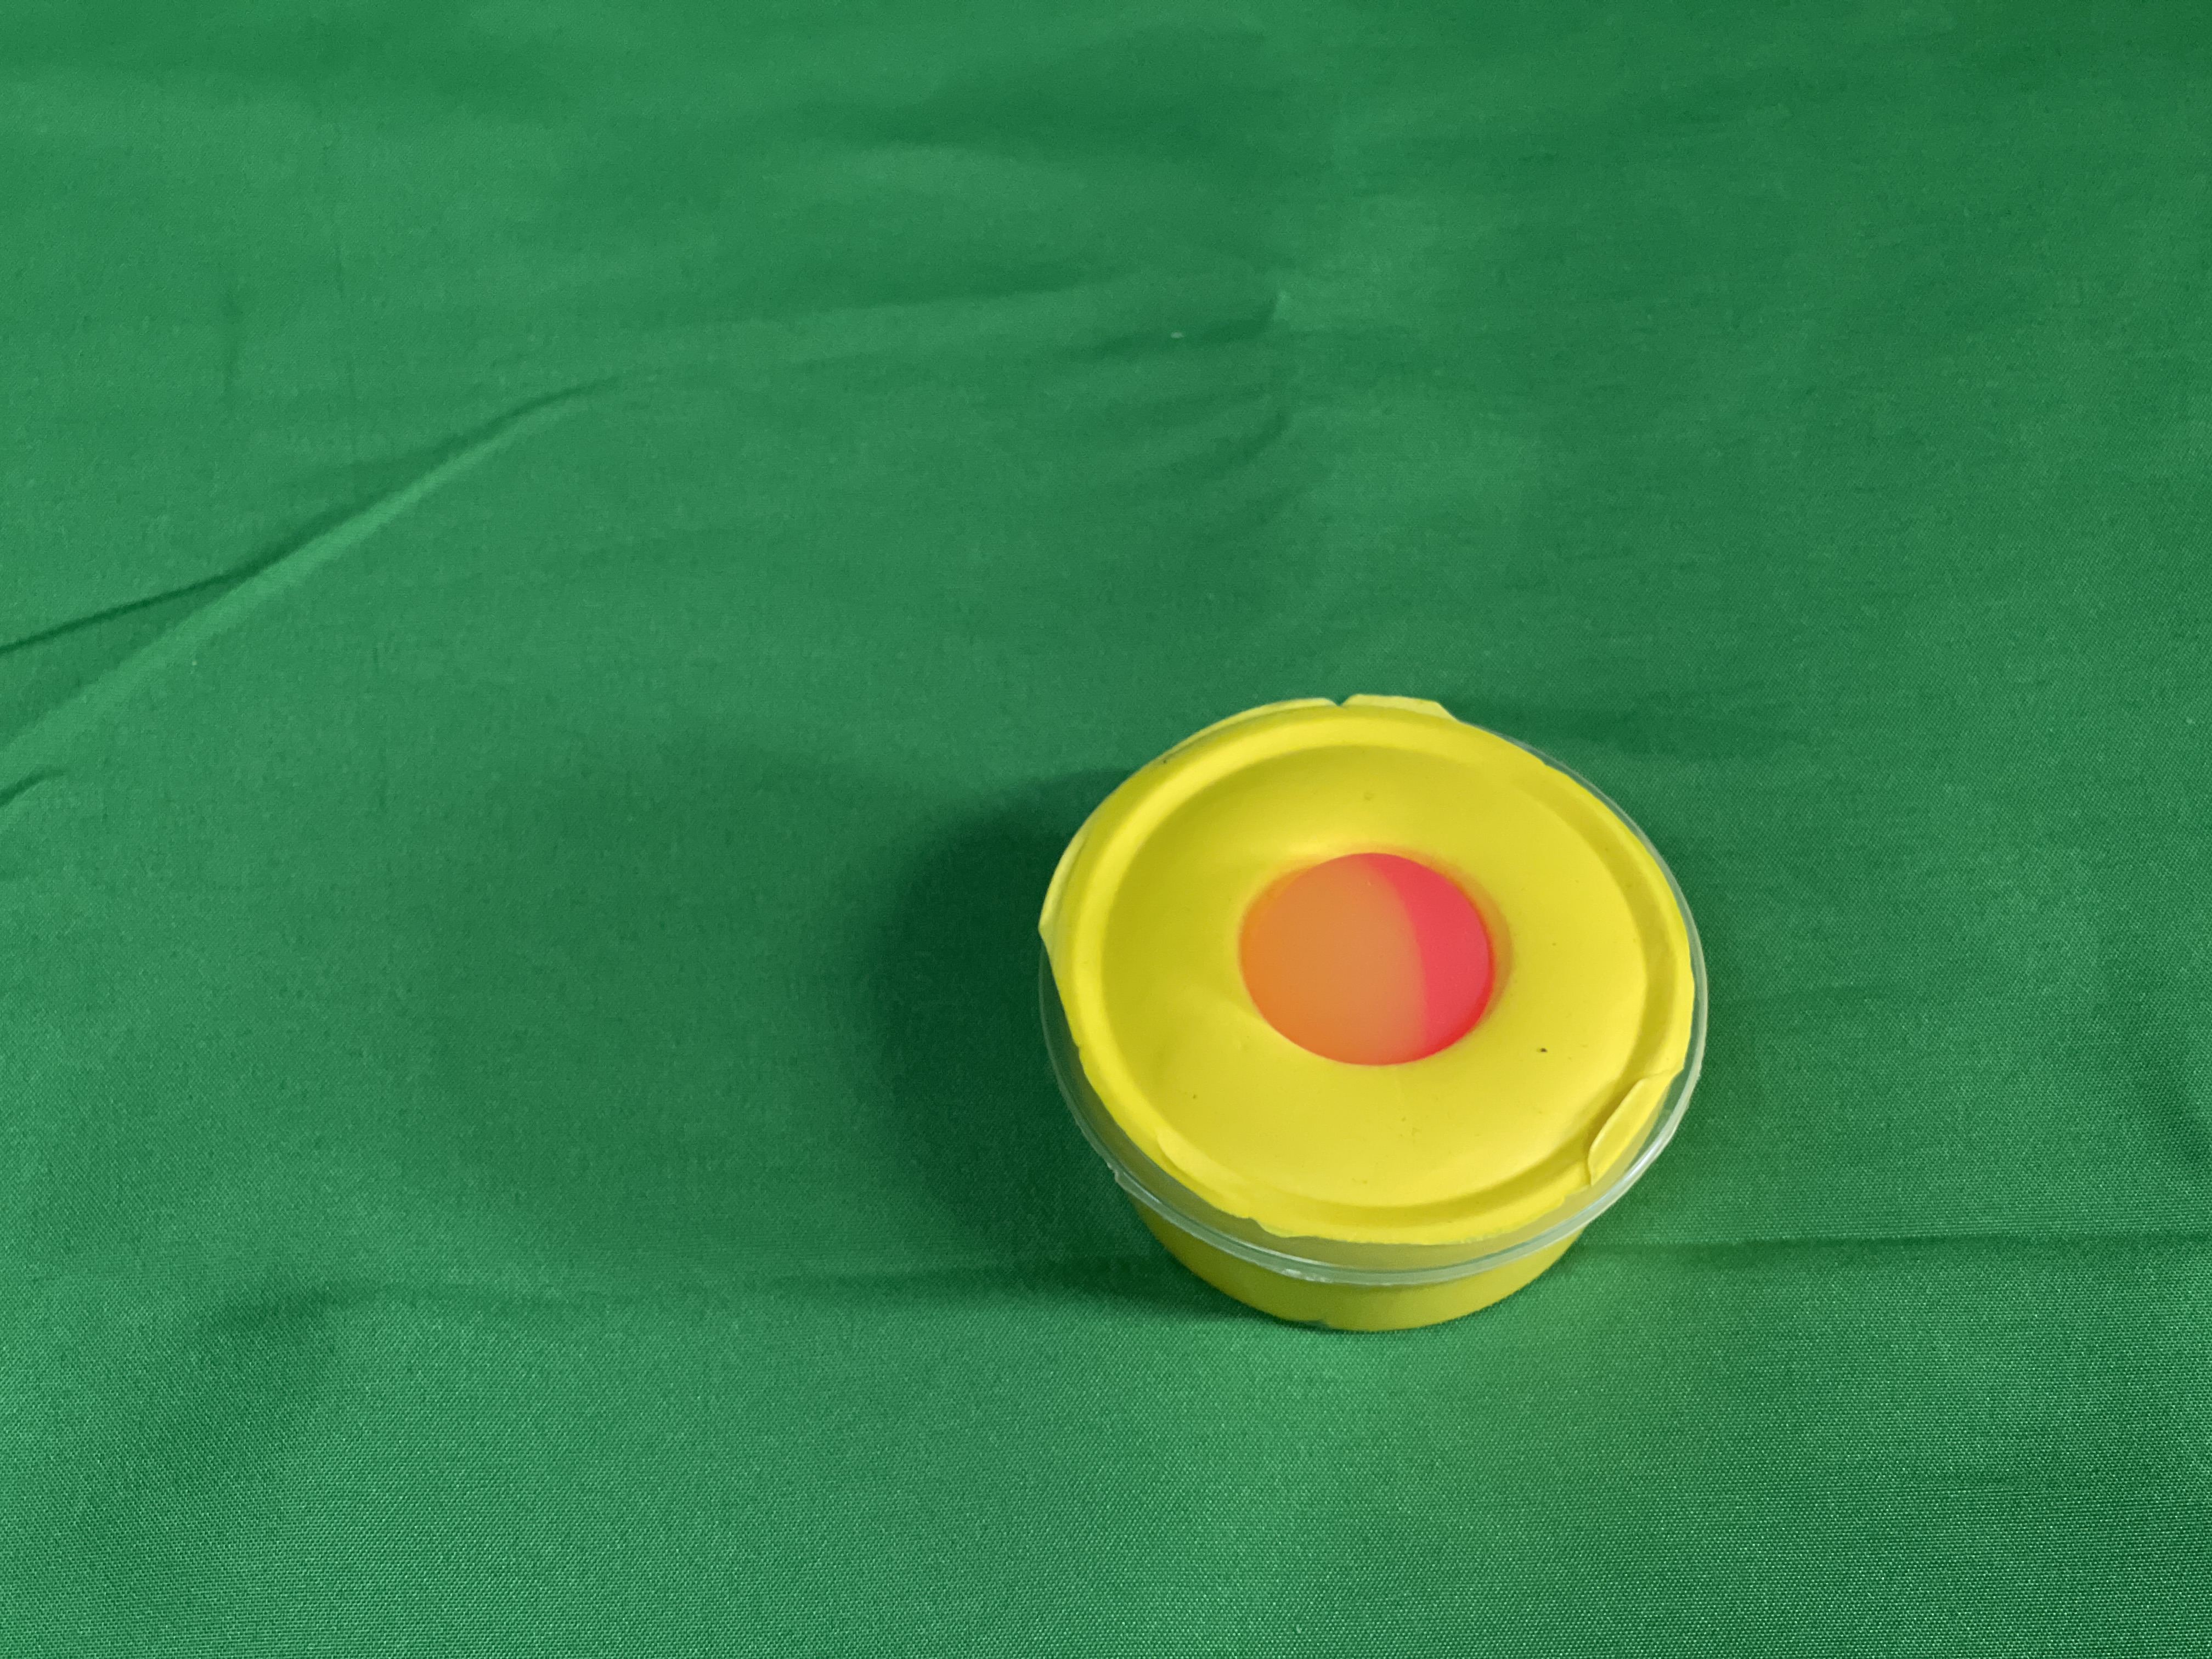
\includegraphics[width=0.22\linewidth]{samples/pb_relationships_motion_general.JPG} \\
\multicolumn{4}{c}{\footnotesize (c) \textbf{Scene} and \textbf{Relationships}}\\
\end{tabular}
\caption{PhysBench Test scenes spanning all four task domains.
Each item poses a 4-way MCQ. Our training distribution overlaps
Property, Dynamics, and Scene; Relationships is not directly represented in
our training data and remains among the weaker domains.}
\label{fig:physbench_grid}
\end{figure}

\end{document}
